\chapter[%
	Ground-State Density Cumulant Theory:\\
	Thermochemical and Kinetic Benchmark Calculations
]{%
	Ground-State Density Cumulant Theory:\\
	Thermochemical and Kinetic Benchmark Calculations\footnote{%
        A.~V.~Copan, A.~Yu.~Sokolov, and H.~F.~Schaefer.,
        J.~Chem.~Theory~Comput.
        {\bfseries 10},
        2389
        (2014).
        Adapted with permission of the American Chemical Society.
    }
}
\label{ch:benchmark}

\section{Abstract}
We present an extensive benchmark study of density cumulant functional theory
(DCFT) for thermochemistry and kinetics of closed- and open-shell molecules. The
performance of DCFT methods (DC-06, DC-12, ODC-06, and ODC-12) is compared to
that of coupled-electron pair methods (CEPA$_0$ and OCEPA$_0$) and
coupled-cluster theory (CCSD and CCSD(T)) for the description of noncovalent
interactions (A24 database), barrier heights of hydrogen-transfer reactions
(HTBH38), radical stabilization energies (RSE30), adiabatic ionization energies
(AIE), and covalent bond stretching in diatomic molecules. Our results indicate
that out of four DCFT methods the ODC-12 method is the most reliable and
accurate DCFT formulation to date. Compared to CCSD, ODC-12 shows superior
results for all benchmark tests employed in our study. With respect to
coupled-pair theories, ODC-12 outperforms CEPA$_0$, and shows similar accuracy
to the orbital-optimized CEPA$_0$ variant (OCEPA$_0$) for systems at equilibrium
geometries. For covalent bond stretching, ODC-12 is found to be more reliable
than OCEPA$_0$. For the RSE30 and AIE datasets, ODC-12 shows competitive
performance with CCSD(T). In addition to benchmark results, we report new
reference values for the RSE30 dataset computed using coupled cluster theory
with up to perturbative quadruple excitations.


\section{Introduction}

Recent developments in {\itshape ab initio} quantum chemistry have resulted in a
variety of computational models for studying molecules.
Apart from concerns about efficiency and accuracy, several concepts have evolved
as criteria for judging the merits of a particular method.
Energy-based criteria typically define an ``ideal'' approximation as one
yielding correlation energies that are size-consistent,
extensive\cite{Nooijen:2005p2277},
well-defined (giving continuous, unique potential surfaces), and
variational.\cite{Pople:1976p1} 
While it has been argued that the practical benefits of variationality are
rather limited,\cite{Bartlett:1981p359} 
the efficiency of gradient computations, at least, is improved by formulating a
theory in terms of a Hermitian and stationary energy
functional.\cite{Szalay:1995p281}
With respect to scope and stability, methods that show consistent performance
for open-shell systems, strongly correlated states, and non-equilibrium
geometries are particularly valuable.\cite{Bartlett:1981p359}

The incorrect scaling of truncated configuration interaction (CI) energies with
system size has inspired the development of size-extensive alternatives. Among
the earliest formulations, the coupled electron pair approximations (CEPAs)
\cite{Kelly:1963p2091,Kelly:1964pA1450,Meyer:1973p1017,Ahlrichs:1979p31,Koch:1981p387}
attracted much attention in
1970s,\cite{Gelus:1970p503,Staemmler:1972p187,Ahlrichs:1975p1235,Kollmar:1977p3583,Wasilewski:1988p1289}
offering rigorous extensivity and size-consistency while retaining much of the
linearity\cite{Taube:2009p1441122} of CI in their equations.
CEPA methods, however, have been shown to rapidly deteriorate as the molecular
geometry deviates from equilibrium\cite{Taube:2009p1441122} and yield energies
that vary under the rotation of the occupied orbitals.\cite{Ahlrichs:1979p31}
Partly in light of such defects, CEPA has been largely displaced by
coupled-cluster (CC)
theory.\cite{Coester:1958p421,Coester:1960p477,Cizek:1966p4256,Bartlett:1978p561,Bartlett:1981p359,Crawford:2000p33,Bartlett:2007p291,Shavitt:2009}
In addition to size-extensivity, CC offers orbital invariance and improved
stability for non-equilibrium structures\cite{Taube:2009p1441122}, but has a
non-Hermitian energy functional and non-linear equations which are not readily
amenable to parallel implementation.
Although neither class of methods is strictly variational, VCEPA (variational
CEPA) has been shown to be effectively equivalent to its non-variational
counterpart.\cite{Kollmar:2010p2449}
Various other modifications to resolve the deficiencies of traditional CEPA have
been explored, including self-consistent size-consistent CI,
\cite{Daudey:1993p1240,Malrieu:2010p179} orbital-invariant CEPA,
\cite{Nooijen:2006p25,Kollmar:2011p084102} and orbital-optimized CEPA
formulations.
\cite{Kollmar:2010p311,Bozkaya:2013p054104,Soydas:2014p1073,Bozkaya:2013p154105}
Recently, the CEPA methods have been revived by Neese and
co-workers\cite{Wennmohs:2008p217,Neese:2009p114108,Kollmar:2010p2449} who
developed the local pair-natural-orbital CEPA (LPNO-CEPA) methods and have
implemented them for massively parallel computer architectures.

It has recently been
demonstrated\cite{Kutzelnigg:2006p171101,Mazziotti:2008p253002,Mazziotti:2010p062515,DePrince:2012p1917}
that CEPA methods naturally arise in the context of theories that obtain the
molecular energies from density cumulants, the connected and extensive
components of the reduced density matrices
(RDMs).\cite{Kutzelnigg:1997p432,Mazziotti:1998p419,Mazziotti:1998p4219,Kutzelnigg:1999p2800,Kong:2011p3541,Hanauer:2012p50}
The advantage of cumulant-based theories is that, unlike their RDM-based
counterparts,\cite{Nakata:2009p042109,vanAggelen:2010p114112,Verstichel:2010p114113}
they are naturally size-extensive and
size-consistent.\cite{Kutzelnigg:1999p2800,Herbert:2007p261}
We have recently achieved the first
implementation\cite{Simmonett:2010p174122,Sokolov:2012p054105} of density
cumulant functional theory (DCFT), proposed by Kutzelnigg in
2006.\cite{Kutzelnigg:2006p171101}
In DCFT, the molecular energy is obtained in terms of a mean-field one-particle
RDM and the two-particle density cumulant, constrained to be at least
approximately $N$-representable ({\it i.e.}\@ to correspond to a physical
$N$-electron wavefunction).
Like traditional CC theory, DCFT is size-extensive and orbital-invariant, but it
has the additional advantage of a stationary and Hermitian energy functional,
which simplifies the computation of molecular properties.
In the original DCFT formulation
(DC-06)\cite{Kutzelnigg:2006p171101,Simmonett:2010p174122,Sokolov:2012p054105}
$N$-representability conditions derived from second-order M\o ller-Plesset
perturbation theory (MPPT) were used,\cite{Kutzelnigg:2004p7350} yielding
equations similar to those of the simplest CEPA model
(CEPA$_0$),\cite{Meyer:1973p1017,Koch:1981p387} but including higher-order terms
in the description of one-particle correlation effects.
Using the same set of conditions, we have developed new formulations of DCFT
that take advantage of an improved description of the one-particle density
matrix (DC-12)\cite{Sokolov:2013p024107} and full orbital optimization (ODC-06
and ODC-12 methods).\cite{Sokolov:2013p204110}

Our previous
studies\cite{Simmonett:2010p174122,Sokolov:2012p054105,Sokolov:2013p024107,Sokolov:2013p204110}
demonstrated for a limited set of systems that the DC-06, DC-12, ODC-06 and
ODC-12 methods generally yield molecular energies and properties competitive
with those obtained by CCSD and CCSD(T), but may exhibit unstable performance
due to imbalances in the description of electron correlation.
Herein, we present an extensive benchmark of the DCFT methods with respect to
thermochemical and kinetic molecular properties, including noncovalent
interactions, barrier heights in hydrogen-transfer reactions, radical
stabilization energies, and adiabatic ionization energies for challenging
electron-dense systems.
We conclude our benchmark study by testing the performance of DCFT for covalent
bond stretching in diatomic molecules.


\section{Overview of DCFT}
In this section a short overview of DCFT is presented. For details on the theory
the reader is referred to our earlier
publications.\cite{Simmonett:2010p174122,Sokolov:2013p024107,Sokolov:2013p204110}
In the RDM methods\cite{Mazziotti:2007} the exact molecular energy is expressed
as a functional of the one- and two-particle reduced density matrices,
$\boldsymbol{\gamma}_1$ and $\boldsymbol{\gamma}_2$ (1-RDM and 2-RDM):
\begin{equation}
	\label{e-rdm}
	E
    = 
	h_p^q
    \gamma_q^p
    +
    \tfrac{1}{2}
    g_{pq}^{rs}
    \gamma_{rs}^{pq} \ ,
	\qquad
	[\boldsymbol{\gamma}_1]_q^p
    \equiv
    \gamma_q^p \ , 
	\qquad
	[\boldsymbol{\gamma}_2]_{rs}^{pq}
    \equiv
    \gamma_{rs}^{pq}\,.
\end{equation}
In \cref{e-rdm}, $h_p^q$ and $g_{pq}^{rs}$ are the usual one- and two-electron
integrals in the orthonormal spin-orbital basis $\{\psi_p\}$ and summation over
the repeated indices is implied.
Expressing $\boldsymbol{\gamma}_1$ through $\boldsymbol{\gamma}_2$ via
the partial trace relation $\sum_r\gamma_{qr}^{pr}=(N-1)\gamma_q^p$, the energy
functional \eqref{e-rdm} can be minimized by varying $\boldsymbol{\gamma}_2$
subject to $N$-representability constraints.
This is the essence of the variational 2-RDM approach.\cite{Mazziotti:2007}


In DCFT, some of the challenges of the 2-RDM approach are circumvented by
expanding $\boldsymbol{\gamma}_2$ in terms of its irreducible components -- the 1-RDM and
the two-particle cumulant (denoted by $\boldsymbol{\lambda}_2$):
\begin{equation}
	\label{lambda}
	\gamma_{rs}^{pq}
    =
	\gamma_r^p
    \gamma_s^q
    -
    \gamma_r^q
    \gamma_s^p
	+
    \lambda_{rs}^{pq}\,.
\end{equation}
In \cref{lambda}, $\boldsymbol{\lambda}_2$ describes the correlated part of $\boldsymbol{\gamma}_2$ that
cannot be expressed via $\boldsymbol{\gamma}_1$. The cumulant also determines the correlation
contribution to $\boldsymbol{\gamma}_1$, allowing the 1-RDM to be decomposed as the sum of an
idempotent 1-RDM ($\boldsymbol{\kappa}$) and a correlation correction ($\boldsymbol{\tau}$):
\begin{equation}
	\label{tau}
	\boldsymbol{\gamma}_1
    =
    \boldsymbol{\kappa}
    +
    \boldsymbol{\tau}\,.
\end{equation}
The correlation component $\boldsymbol{\tau}$ is fully specified by $\boldsymbol{\lambda}_2$, whereas
$\boldsymbol{\kappa}$ is independent of $\boldsymbol{\lambda}_2$. \Cref{lambda,tau} allow us to write an
equivalent energy expression with $\boldsymbol{\kappa}$ and $\boldsymbol{\lambda}_2$ as independent
functional parameters:
\begin{equation}
	\label{e-dcft}
    \begin{array}{c}
        E[\boldsymbol{\kappa},\boldsymbol{\lambda}_2]
        =
        \tfrac{1}{2}
        (h_p^q+f_p^q)
        (\kappa_q^p+\tau_q^p)
        +
        \tfrac{1}{4}
        \overline{g}_{pq}^{rs}
        \lambda_{pq}^{rs}
        ,
        \\
        f_p^q
        =
        h_p^q
        +
        \overline{g}_{pr}^{qs}
        (\kappa_s^r+\tau_s^r)
        ,
        \quad
        \overline{g}_{rs}^{pq}
        =
        g_{rs}^{pq}
        -
        g_{rs}^{qp}\,.
    \end{array}
\end{equation}
Here, the generalized Fock operator $\boldsymbol{f}$ differs from that of
Hartree-Fock theory by the presence of an external potential
$\overline{g}_{pr}^{qs}\tau_s^r$ due to electron
correlation.\cite{Kutzelnigg:2006p171101}


To date, all DCFT formulations make the energy (\ref{e-dcft}) stationary with
respect to variations of $\boldsymbol{\lambda}_2$, subject to cumulant
$N$-representability constraints derived from second-order M\o ller-Plesset
perturbation theory (MPPT).\cite{Kutzelnigg:2004p7350}
To account for orbital relaxation effects, the two earliest DCFT methods,
DC-06\cite{Kutzelnigg:2006p171101,Simmonett:2010p174122,Sokolov:2012p054105} and
DC-12\cite{Sokolov:2013p024107}, determined the orbitals by diagonalizing the
generalized Fock operator $\boldsymbol{f}$ defined in \cref{e-dcft}.
These two methods differ in their description of 1-RDM $N$-representability.
Whereas DC-06 employs an approximate expression for $\boldsymbol{\tau}$ in terms
of $\boldsymbol{\lambda}_2$, DC-12 uses the exact relationship.
Recently, we proposed orbital-optimized variants of DC-06 and DC-12 (ODC-06 and
ODC-12),\cite{Sokolov:2013p204110} which fully account for orbital relaxation
effects.


\section{Computational Details}


All computations were performed using the Psi4
package.\cite{Turney:2012p556}
The results were benchmarked against coupled cluster theory with single and
double excitations (CCSD)\cite{Crawford:2000p33,Bartlett:2007p291,Shavitt:2009},
CCSD with perturbative triple excitations
[CCSD(T)],\cite{Raghavachari:1989p479,Stanton:1997p130} coupled electron pair
approximation zero (CEPA$_0$),\cite{Meyer:1973p1017,Koch:1981p387} and the
orbital-optimized variant of CEPA$_0$ (OCEPA$_0$)\cite{Bozkaya:2013p054104}.
All electrons were correlated in all computations.
The cc-pCVXZ\cite{Dunning:1989p1007,Woon:1995p4572} and
aug-cc-pVXZ\cite{Kendall:1992p6796} basis sets (X = T, Q) were used (see text
for details).
Noncovalent interaction energies, hydrogen-transfer barrier heights, and radical
stabilization energies were computed using geometries from the
A24\cite{Rezac:2013p2151}, HTBH38\cite{Zhao:2005p43}, and
RSE30\cite{Soydas:2013p1452} benchmark databases, respectively, available in
Psi4.
Adiabatic ionization energies were computed from neutral and cation geometries
optimized at each level of theory, with added harmonic zero-point vibrational
energy corrections.
Harmonic frequencies were computed by numerical differentiation of analytic
energy gradients.
Single-point energies were converged to $10^{-8}$~\hartree, while the root mean
square of the energy gradient was converged to $10^{-6}$~\hartree/\bohr for
geometry optimizations. 


\section{Results}

\subsection{Noncovalent Interactions}

\afterpage{%
    \clearpage
    \centering
    \begin{landscape}
        \vspace*{\fill}
        \captionof{table}{%
            \label{a24-t}
            Errors in interaction energies (\kcal) for 24 noncovalently
            bound molecular dimers comprising the A24
            database\cite{Rezac:2013p2151} computed using seven methods with
            the aug-cc-pVTZ basis set.
            The errors are relative to CCSD(T) reference values (\kcal)
            shown in the rightmost column.
            For each method the mean absolute deviations from CCSD(T) (\mae,
            \kcal) and the standard deviations from the mean signed error
            (\std, \kcal) are also shown.
        }
        \small
        \renewcommand\arraystretch{0.6}
        \begin{tabular}{c@{}rrrrrrrr}
            \hline
            \hline
            Complex (Sym.) &
            $\Delta$CEPA$_0$ &  $\Delta$DC-06 & $\Delta$DC-12 &
            $\Delta$CCSD & $\Delta$OCEPA$_0$ & $\Delta$ODC-06 &
            $\Delta$ODC-12 &
            CCSD(T)
            \\
            \hline
            \ce{H2O\bond{...}NH3} (\termsymbol{C_{s}}) &
            0.26 & 0.24 & 0.22 &  0.36 & 0.19 & 0.20 & 0.18 & 
            -7.18\\
            \ce{H2O\bond{...}H2O} (\termsymbol{C_{s}}) &
            0.19 & 0.18 & 0.16 &  0.25 & 0.13 & 0.14 & 0.12 & 
            -5.71\\
            \ce{HCN\bond{...}HCN} (\termsymbol{C_{s}}) &
            0.21 & 0.27 & 0.16 &  0.15 & 0.18 & 0.26 & 0.14 & 
            -7.12\\
            \ce{HF\bond{...}HF} (\termsymbol{C_{s}}) &
            0.14 & 0.13 & 0.11  & 0.16 & 0.08 & 0.09 & 0.07 & 
            -5.20\\
            \ce{NH3\bond{...}NH3} (\termsymbol{C_{2h}}) &
            0.15 & 0.13 & 0.14 &  0.26 & 0.12 & 0.12 & 0.12 & 
            -3.43\\
            \ce{HF\bond{...}CH4} (\termsymbol{C_{3v}}) &
            0.17 & 0.16 & 0.20 &  0.23 & 0.12 & 0.12 & 0.16 & 
            -2.30\\
            \ce{NH3\bond{...}CH4} (\termsymbol{C_{3v}}) &
            0.07 & 0.05 & 0.05 &  0.13 & 0.05 & 0.05 & 0.04 & 
            -1.08\\
            \ce{H2O\bond{...}CH4} (\termsymbol{C_{s}}) &
            0.06 & 0.05 & 0.04 &  0.11 & 0.05 & 0.05 & 0.04 & 
            -1.03\\
            \ce{CH2O\bond{...}CH2O} (\termsymbol{C_{s}}) &
            0.89 & 0.99 & 0.65 &  0.46 & 0.62 & 0.87 & 0.46 & 
            -5.23\\
            \ce{H2O\bond{...}C2H4} (\termsymbol{C_{s}}) &
            0.15 & 0.16 & 0.15 &  0.31 & 0.20 & 0.26 & 0.21 & 
            -3.33\\
            \ce{CH2O\bond{...}C2H4} (\termsymbol{C_{s}}) &
            0.21 & 0.18 & 0.14 &  0.27 & 0.19 & 0.24 & 0.16 & 
            -2.24\\
            \ce{HCCH\bond{...}HCCH} (\termsymbol{C_{2v}}) &
            0.07 & 0.05 & 0.05 &  0.20 & 0.10 & 0.12 & 0.10 & 
            -2.57\\
            \hline
            \hline
        \end{tabular}
        \vspace*{\fill}
        \newpage
        \vspace*{\fill}
        \begin{tabular}{c@{}rrrrrrrr}
            \hline
            \hline
            Complex (Sym.) &
            $\Delta$CEPA$_0$ &  $\Delta$DC-06 & $\Delta$DC-12 &
            $\Delta$CCSD & $\Delta$OCEPA$_0$ & $\Delta$ODC-06 &
            $\Delta$ODC-12 &
            CCSD(T)
            \\
            \hline
            \ce{NH3\bond{...}C2H4} (\termsymbol{C_{s}}) &
            0.09 & 0.06 & 0.08 &  0.24 & 0.12 & 0.15 & 0.13 & 
            -2.07\\
            \ce{C2H4\bond{...}C2H4} (\termsymbol{C_{2v}}) &
            0.10 & 0.02 & 0.07 &  0.33 & 0.14 & 0.13 & 0.15 & 
            -1.81\\
            \ce{CH4\bond{...}C2H4} (\termsymbol{C_{s}}) &
            0.02 & -0.02 & 0.01 &  0.14 & 0.05 & 0.04 & 0.06 & 
            -0.92\\
            \ce{BH3\bond{...}CH4} (\termsymbol{C_{s}}) &
            0.23 & 0.18 & 0.24 &  0.37 & 0.18 & 0.16 & 0.22 & 
            -2.52\\
            \ce{CH4\bond{...}C2H4} (\termsymbol{C_{s}}) &
            0.13 & 0.09 & 0.13 &  0.23 & 0.10 & 0.09 & 0.09 & 
            -1.37\\
            \ce{CH4\bond{...}C2H6} (\termsymbol{C_{s}}) &
            0.09 & 0.06 & 0.09 &  0.17 & 0.07 & 0.06 & 0.09 & 
            -1.14\\
            \ce{CH4\bond{...}CH4} (\termsymbol{D_{3d}}) &
            0.08 & 0.06 & 0.08 &  0.14 & 0.06 & 0.05 & 0.08 & 
            -0.93\\
            \ce{Ar\bond{...}CH4} (\termsymbol{C_{3v}}) &
            0.07 & 0.05 & 0.07 &  0.10 & 0.05 & 0.05 & 0.06 & 
            -0.78\\
            \ce{Ar\bond{...}C2H4} (\termsymbol{C_{2v}}) &
            0.03 & -0.01 & 0.02 &  0.11 & 0.05 & 0.03 & 0.05 & 
            -0.63\\
            \ce{C2H4\bond{...}HCCH} (\termsymbol{C_{2v}}) &
            -0.02 & -0.19 & -0.01 &  0.38 & 0.07 & -0.06 & 0.11 & 
            0.43\\
            \ce{C2H4\bond{...}C2H4} (\termsymbol{D_{2h}}) &
            -0.05 & -0.30 & -0.03 &  0.43 & 0.04 & -0.16 & 0.11 & 
            0.41\\
            \ce{HCCH\bond{...}HCCH} (\termsymbol{D_{2h}}) &
            0.01 & -0.09 & 0.02 &  0.34 & 0.10 & 0.02 & 0.12 & 
            0.91\\
            \hline
            \mae: &
            0.14 & 0.16 & 0.12 & 0.25 & 0.13 & 0.15 & 0.13 &
            \\
            \std: &
            0.18 & 0.23 & 0.13 & 0.11 & 0.12 & 0.18 & 0.09 &
            \\
            \hline
            \hline
        \end{tabular}
        \vspace*{\fill}
    \end{landscape}
    \newpage
    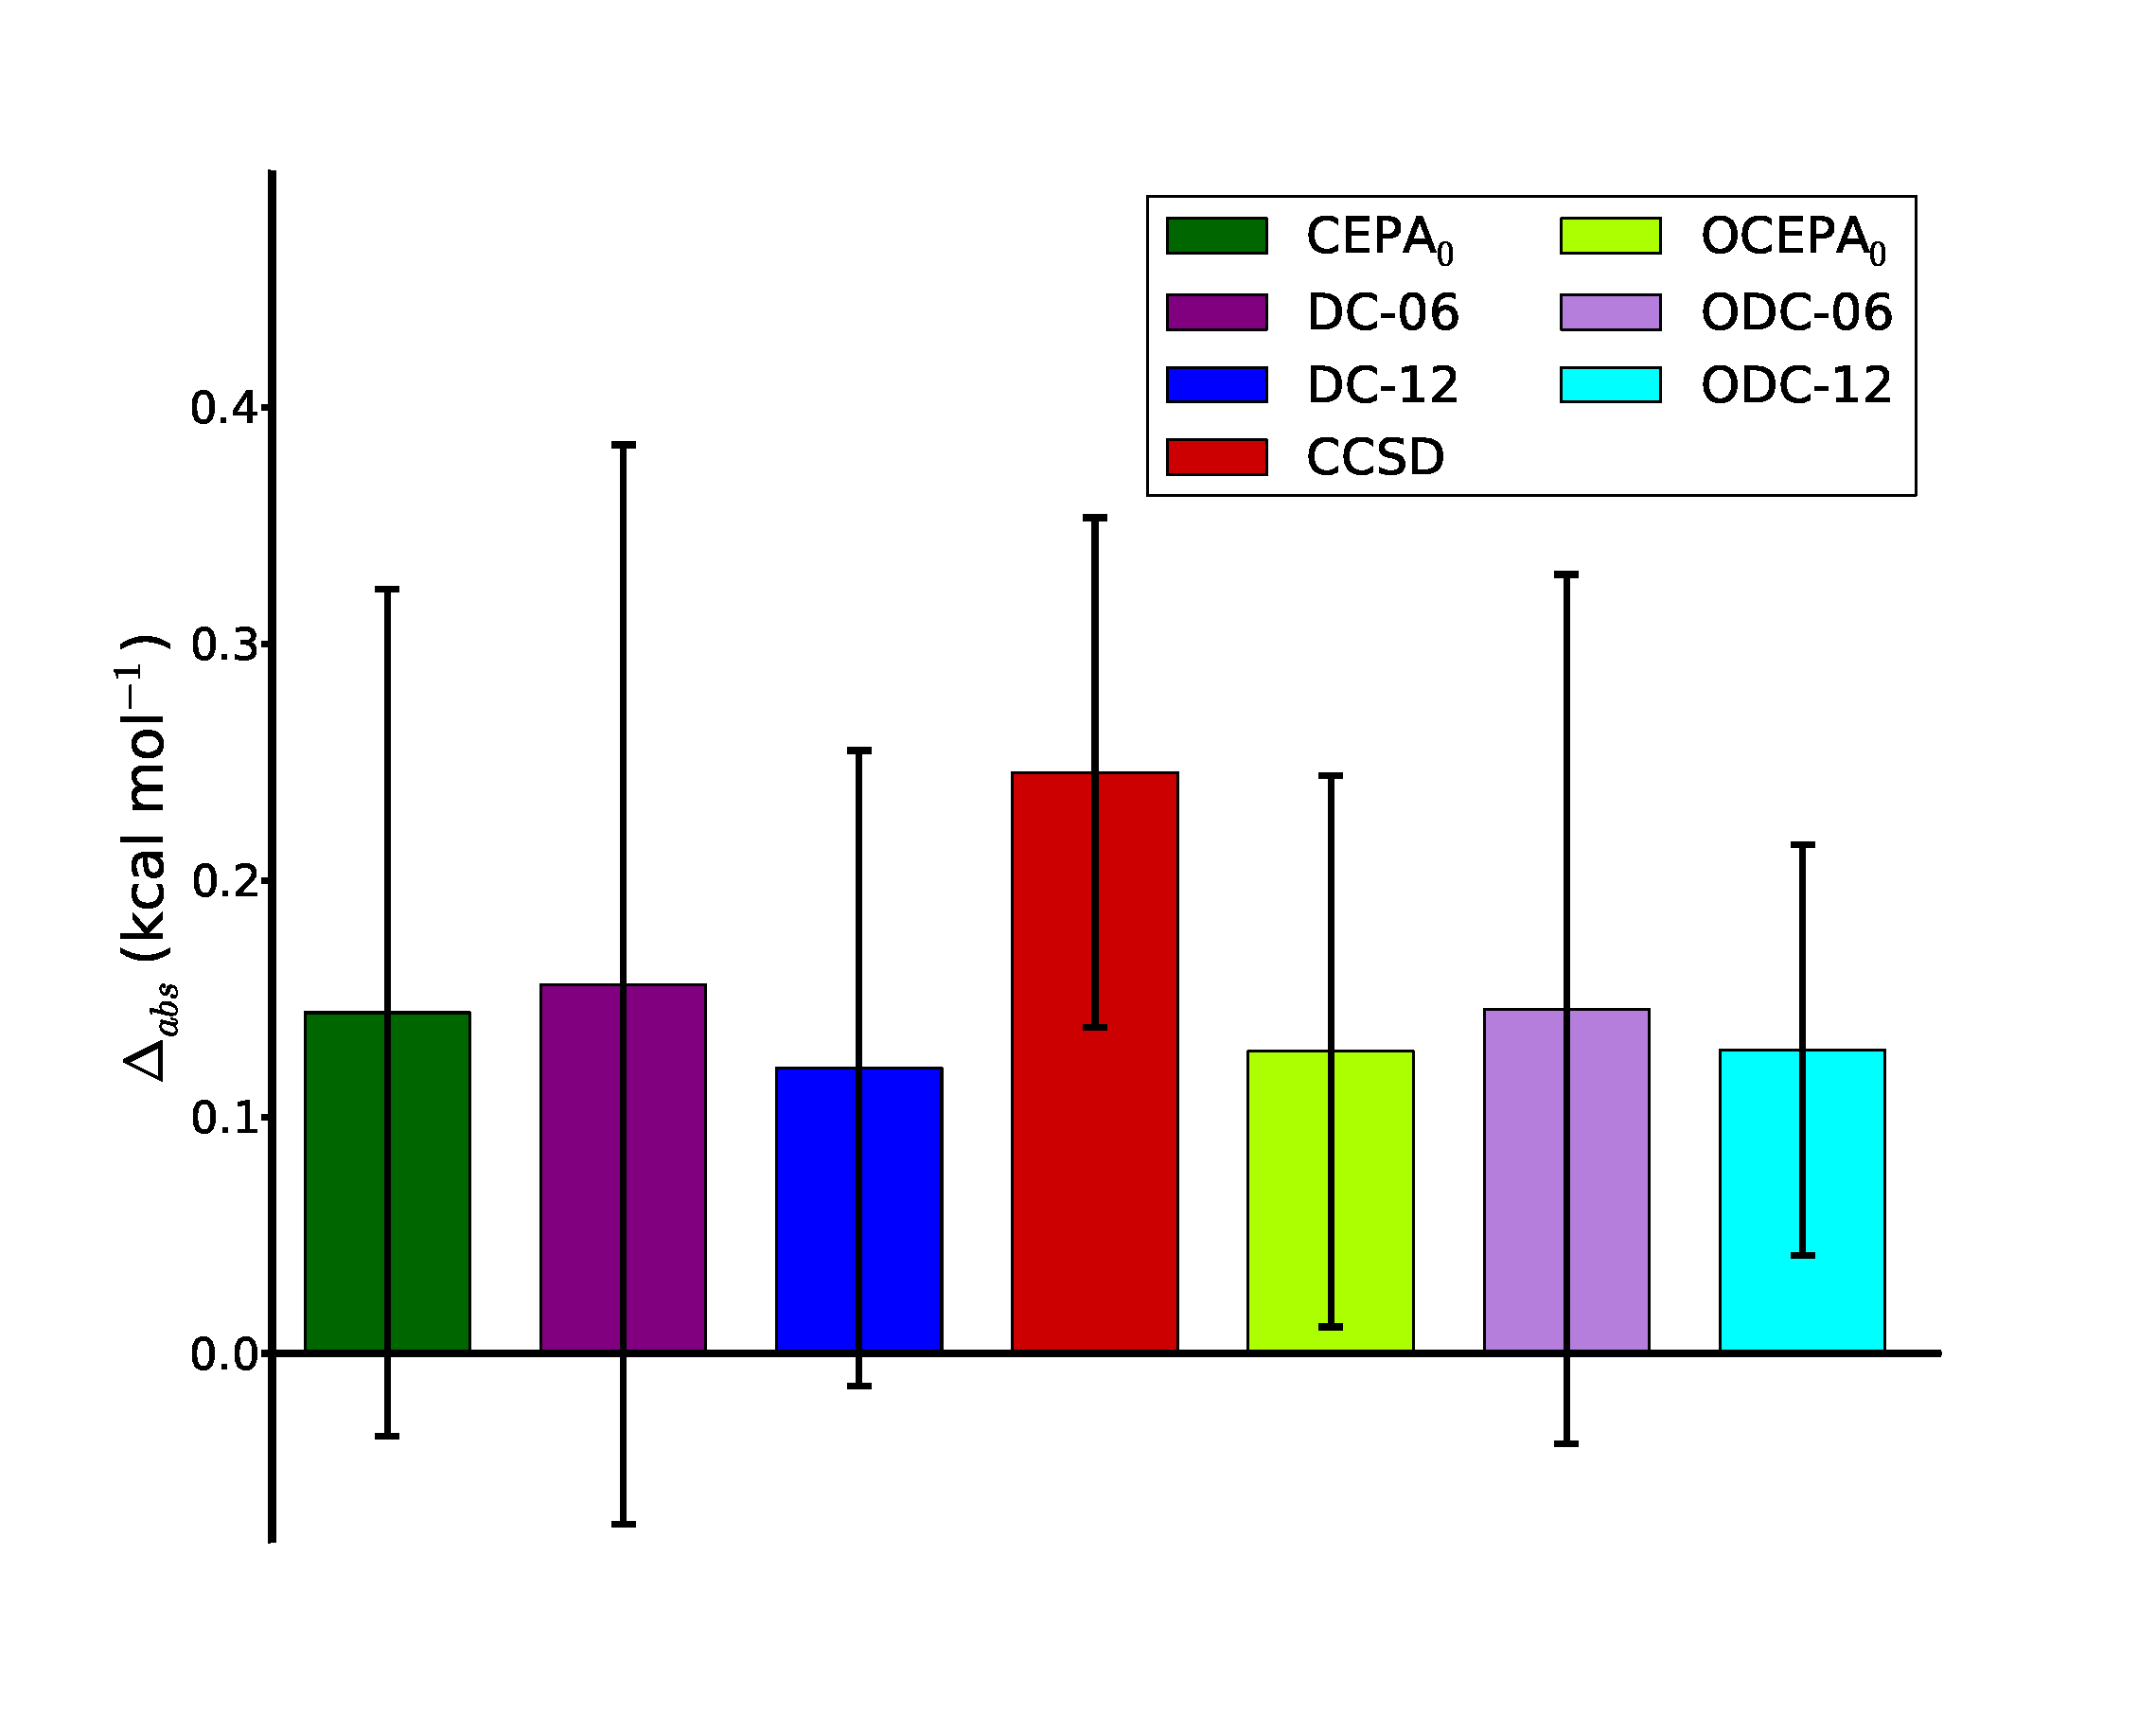
\includegraphics[width=0.8\textwidth]{figures/a24.pdf}
    \captionof{figure}{%
        \label{a24-f}
        Mean absolute deviations (\mae, \kcal) and the standard deviations
        from the mean signed error (\std, \kcal) of the interaction energies
        for 24 noncovalently bound molecular dimers (A24 database) computed
        using seven methods with the aug-cc-pVTZ basis set.
        The errors are relative to CCSD(T)/aug-cc-pVTZ reference values.
        The \mae value is represented as a height of each colored box, while
        the \std value is depicted as a radius of the black vertical bar.
        See \cref{a24-t} for data on individual database members.
    }
}


We begin by testing the accuracy of DCFT methods for the description of
noncovalent interactions in 24 closed-shell molecular dimers, which are listed
in \cref{a24-t}.
These molecular complexes comprise the A24 dataset\cite{Rezac:2013p2151}
developed by \v{R}ez\'a\v{c} and Hobza to include a variety of noncovalent
interactions, including hydrogen bonding and $\pi$-$\pi$ stacking.
Although \v{R}ez\'a\v{c} and Hobza reported the interaction energies at the
CCSD(T) complete basis set (CBS) limit, we use CCSD(T)/aug-cc-pVTZ energies as
reference values in order to effectively exclude basis-set incompleteness error
from the comparison.

\Cref{a24-f} depicts mean absolute error (\mae) relative to CCSD(T) in the
binding energies of CEPA$_0$, OCEPA$_0$, CCSD, and the four DCFT methods (DC-06,
DC-12, ODC-06, and ODC-12), as well as the root mean square deviation from the
average signed error (\std).
All methods but CCSD give similar \mae values ($0.14\pm 0.02$~\kcal), and a
comparison between CEPA$_0$, DC-06, and DC-12 and their orbital-optimized
variants (OCEPA$_0$, ODC-06, and ODC-12) shows negligible 0.01~\kcal differences
in each case.
CCSD gives a significantly larger \mae (0.25~\kcal) than the other methods,
exceeding the DC-12 \mae by a factor of two (0.12~\kcal).
The \std values are much more sensitive to the choice of method than the \mae
values, and are noticeably affected by orbital optimization.
ODC-12 gives the smallest standard deviation (\std = 0.09~\kcal), while the
largest \std value was found for DC-06 (0.23~\kcal). The OCEPA$_0$, ODC-06, and
ODC-12 methods (\std = 0.12, 0.18, and 0.09~\kcal, respectively) exhibit much
more consistent performance than their non-orbital-optimized analogues, with
\std smaller by $0.05\pm 0.01$~\kcal in each case.
CCSD also exhibits a relatively small \std value ($0.11$~\kcal), possibly due to
its inclusion of single excitations which partly account for orbital relaxation.

Errors in interaction energy and CCSD(T) reference values for each molecular
complex are shown in \cref{a24-t}.
The largest deviations from CCSD(T) were obtained for the formaldehyde dimer
($\mathrm{CH_2O }\cdots\mathrm{CH_2O }$, complex 9 in \cref{a24-t}), for which
DC-06, CEPA$_0$, and OCEPA$_0$ yield errors of 0.99, 0.89, and 0.87~\kcal,
respectively.
For this system, the best performance is shown by CCSD and ODC-12, both of which
give an error of 0.46~\kcal.
For systems with $\pi$-stacking interactions (complexes 22-24 in \cref{a24-t}),
CCSD shows large errors (0.38, 0.43, 0.34~\kcal) relative to the magnitude of
the interaction energy (0.43, 0.41, 0.91~\kcal, respectively).
Here CEPA$_0$, DC-12, and their orbital-optimized variants offer much better
agreement with CCSD(T), with errors ranging from 0.01 to 0.15 \kcal.


\subsection{Hydrogen-Transfer Reaction Barrier Heights}

\afterpage{%
    \clearpage
    \centering
    \begin{landscape}
        \vspace*{\fill}
        \captionof{table}{%
            \label{htbh-t}
            Errors in barrier heights (\kcal) for 18 hydrogen-transfer
            reactions (\ce{R1 + R2H $\rightarrow$ R1H + R2}) comprising the
            HTBH38 database\cite{MN-Database} computed using five methods
            with the aug-cc-pVTZ basis set.
            The errors are relative to CCSD(T) reference values (\kcal)
            shown in the rightmost column.
            Each reaction includes barrier heights in the forward (\ce{R1 +
            R2H $\rightarrow$ [R1R2H]^*}) and reverse (\ce{[R1R2H]^*
            $\leftarrow$ R1H + R2}) directions, respectively, except in the
            case of \(\ce{R1} = \ce{R2} = H\) where they are the same.
            The mean absolute (\mae, \kcal) and the mean percent (\rel, \%)
            errors with respect to CCSD(T), as well as the standard
            deviations from the mean signed error (\std, \kcal) are also
            shown.
        }
        \vspace{1em}
        \renewcommand\arraystretch{0.6}
        \begin{tabular}{lcrrrrrr}
            \hline
            \hline
            &
            Reaction Barrier &
            $\Delta$CEPA$_0$ &  $\Delta$DC-12 &   $\Delta$CCSD &
            $\Delta$OCEPA$_0$ & $\Delta$ODC-12 &
            CCSD(T)
            \\
            \hline
            1 & \ce{H + HCl  $\rightarrow$ [HHCl]^*} &
            0.74 & 0.49 & 0.09 & -0.41 & -0.28 & 5.22 \\
            2 &\ce{OH + H2  $\rightarrow$ [OHH2]^*} &
            3.77 & 3.38 & 1.82 & 0.88 & 1.24 & 4.99 \\
            3 &\ce{CH3 + H2  $\rightarrow$ [CH3H2]^*} &
            1.60 & 1.46 & 1.37 & 0.46 & 0.70 & 11.29 \\
            4 &\ce{OH + CH4  $\rightarrow$ [OHCH4]^*} &
            4.26 & 3.85 & 2.61 & 1.22 & 1.65 & 5.64 \\
            5 &\ce{H + H2  $\rightarrow$ [HH2]^*} &
            0.80 & 0.69 & 0.30 & -0.27 & -0.05 & 9.77 \\
            6 &\ce{OH + NH3  $\rightarrow$ [OHNH3]^*} &
            6.02 & 5.25 & 3.54 & 1.18 & 1.82 & 3.17 \\
            7 &\ce{HCl + CH3  $\rightarrow$ [HClCH3]^*} &
            1.93 & 1.78 & 1.79 & 0.68 & 0.92 & 0.10 \\
            8 &\ce{OH + C2H6  $\rightarrow$ [OHC2H6]^*}
            & 4.66 & 4.21 & 2.69 & 1.28 & 1.72 & 2.69 \\
            9 &\ce{F + H2  $\rightarrow$ [FH2]^*} &
            3.40 & 3.14 & 1.20 & 0.52 & 0.78 & 1.13 \\
            10 &\ce{O + CH4  $\rightarrow$ [OHCH3]^*} &
            3.40 & 3.12 & 2.37 & 0.70 & 1.20 & 13.62 \\
            11 &\ce{H + PH3  $\rightarrow$ [HPH3]^*} &
            0.93 & 0.86 & 0.59 & -0.16 & 0.10 & 2.29 \\
            12 &\ce{H + HO  $\rightarrow$ [OHH]^*} &
            2.03 & 1.59 & 0.44 & -0.61 & -0.26 & 10.25 \\
            13 &\ce{H + H2S  $\rightarrow$ [HH2S]^*} &
            1.01 & 0.92 & 0.65 & -0.11 & 0.14 & 3.17 \\
            14 &\ce{O + HCl  $\rightarrow$ [OHCl]^*} &
            6.33 & 6.01 & 3.58 & 0.79 & 1.51 & 9.74 \\
            15 &\ce{NH2 + CH3  $\rightarrow$ [CH3NH2]^*} &
            2.48 & 2.22 & 1.99 & 0.49 & 0.86 & 7.66 \\
            16 &\ce{NH2 + C2H5  $\rightarrow$ [NH2C2H5]^*} &
            2.48 & 2.22 & 2.09 & 0.55 & 0.92 & 8.21 \\
            17 &\ce{C2H6 + NH2  $\rightarrow$ [C2H6NH2]^*} &
            3.30 & 3.00 & 2.73 & 1.23 & 1.62 & 10.39 \\
            18 &\ce{NH2 + CH4  $\rightarrow$ [NH2CH4]^*} &
            2.98 & 2.72 & 2.55 & 1.11 & 1.48 & 13.23 \\
            \hline
        \end{tabular}
        \vspace*{\fill}
        \newpage
        \vspace*{\fill}
        \begin{tabular}{lcrrrrrr}
            \hline
            \hline
            &
            Reaction Barrier &
            $\Delta$CEPA$_0$ &  $\Delta$DC-12 &   $\Delta$CCSD &
            $\Delta$OCEPA$_0$ & $\Delta$ODC-12 &
            CCSD(T)
            \\
            \hline
            1 & \ce{[HHCl]^* $\leftarrow$  H2 + Cl} &
            1.44 & 1.31 & 1.61 & 0.53 & 0.77 & 7.39 \\
            2 &\ce{[OHH2]^* $\leftarrow$  H + H2O} &
            2.09 & 1.66 & 0.09 & -0.91 & -0.58 & 21.07 \\
            3 &\ce{[CH3H2]^* $\leftarrow$  H + CH4} &
            0.95 & 0.80 & 0.38 & -0.38 & -0.11 & 14.91 \\
            4 &\ce{[OHCH4]^* $\leftarrow$  CH3 + H2O} &
            3.23 & 2.80 & 1.87 & 0.27 & 0.65 & 18.09 \\
            6 &\ce{[OHNH3]^* $\leftarrow$  H2O + NH2} &
            5.46 & 4.62 & 3.14 & 0.79 & 1.33 & 13.17 \\
            7 &\ce{[HClCH3]^* $\leftarrow$  Cl + CH4} &
            1.97 & 1.94 & 2.31 & 0.78 & 1.16 & 5.89 \\
            8 &\ce{[OHC2H6]^* $\leftarrow$  H2O + C2H5} &
            3.34 & 2.89 & 1.85 & 0.28 & 0.64 & 18.49 \\
            9 &\ce{[FH2]^* $\leftarrow$  HF + H} &
            1.27 & 0.88 & -0.78 & -1.47 & -1.33 & 32.95 \\
            10 &\ce{[OHCH3]^* $\leftarrow$  OH + CH3} &
            2.62 & 2.29 & 1.82 & 0.32 & 0.68 & 7.43 \\
            11 &\ce{[HPH3]^* $\leftarrow$  PH2 + H2} &
            1.14 & 1.11 & 1.37 & 0.39 & 0.63 & 23.21 \\
            12 &\ce{[OHH]^* $\leftarrow$  H2 + O} &
            3.47 & 3.08 & 1.99 & 0.62 & 1.07 & 12.81 \\
            13 &\ce{[HH2S]^* $\leftarrow$  H2 + HS} &
            1.51 & 1.51 & 1.88 & 0.65 & 0.97 & 16.41 \\
            14 &\ce{[OHCl]^* $\leftarrow$  OH + Cl} &
            5.59 & 5.35 & 3.55 & 0.51 & 1.24 & 9.35 \\
            15 &\ce{[CH3NH2]^* $\leftarrow$  CH4 + NH} &
            2.77 & 2.49 & 2.26 & 0.73 & 1.12 & 21.32 \\
            16 &\ce{[NH2C2H5]^* $\leftarrow$  C2H6 + NH} &
            3.06 & 2.75 & 2.46 & 0.85 & 1.26 & 18.52 \\
            17 &\ce{[C2H6NH2]^* $\leftarrow$  NH3 + C2H5} &
            2.54 & 2.30 & 2.30 & 0.63 & 1.02 & 16.20 \\
            18 &\ce{[NH2CH4]^* $\leftarrow$  CH3 + NH3} &
            2.51 & 2.29 & 2.21 & 0.56 & 0.96 & 15.69
            \\
            \hline
            &
            \mae: &
            2.77 & 2.49 & 1.84 & 0.67 & 0.94 &
            \\
            &
            \std: &
            1.51 & 1.39 & 1.06 & 0.62 & 0.71 &
            \\
            &
            \rel \%: &
            99 & 90 & 77 & 29 & 40
            \\
            \hline
            \hline
        \end{tabular}
        \vspace*{\fill}
    \end{landscape}
    \newpage
    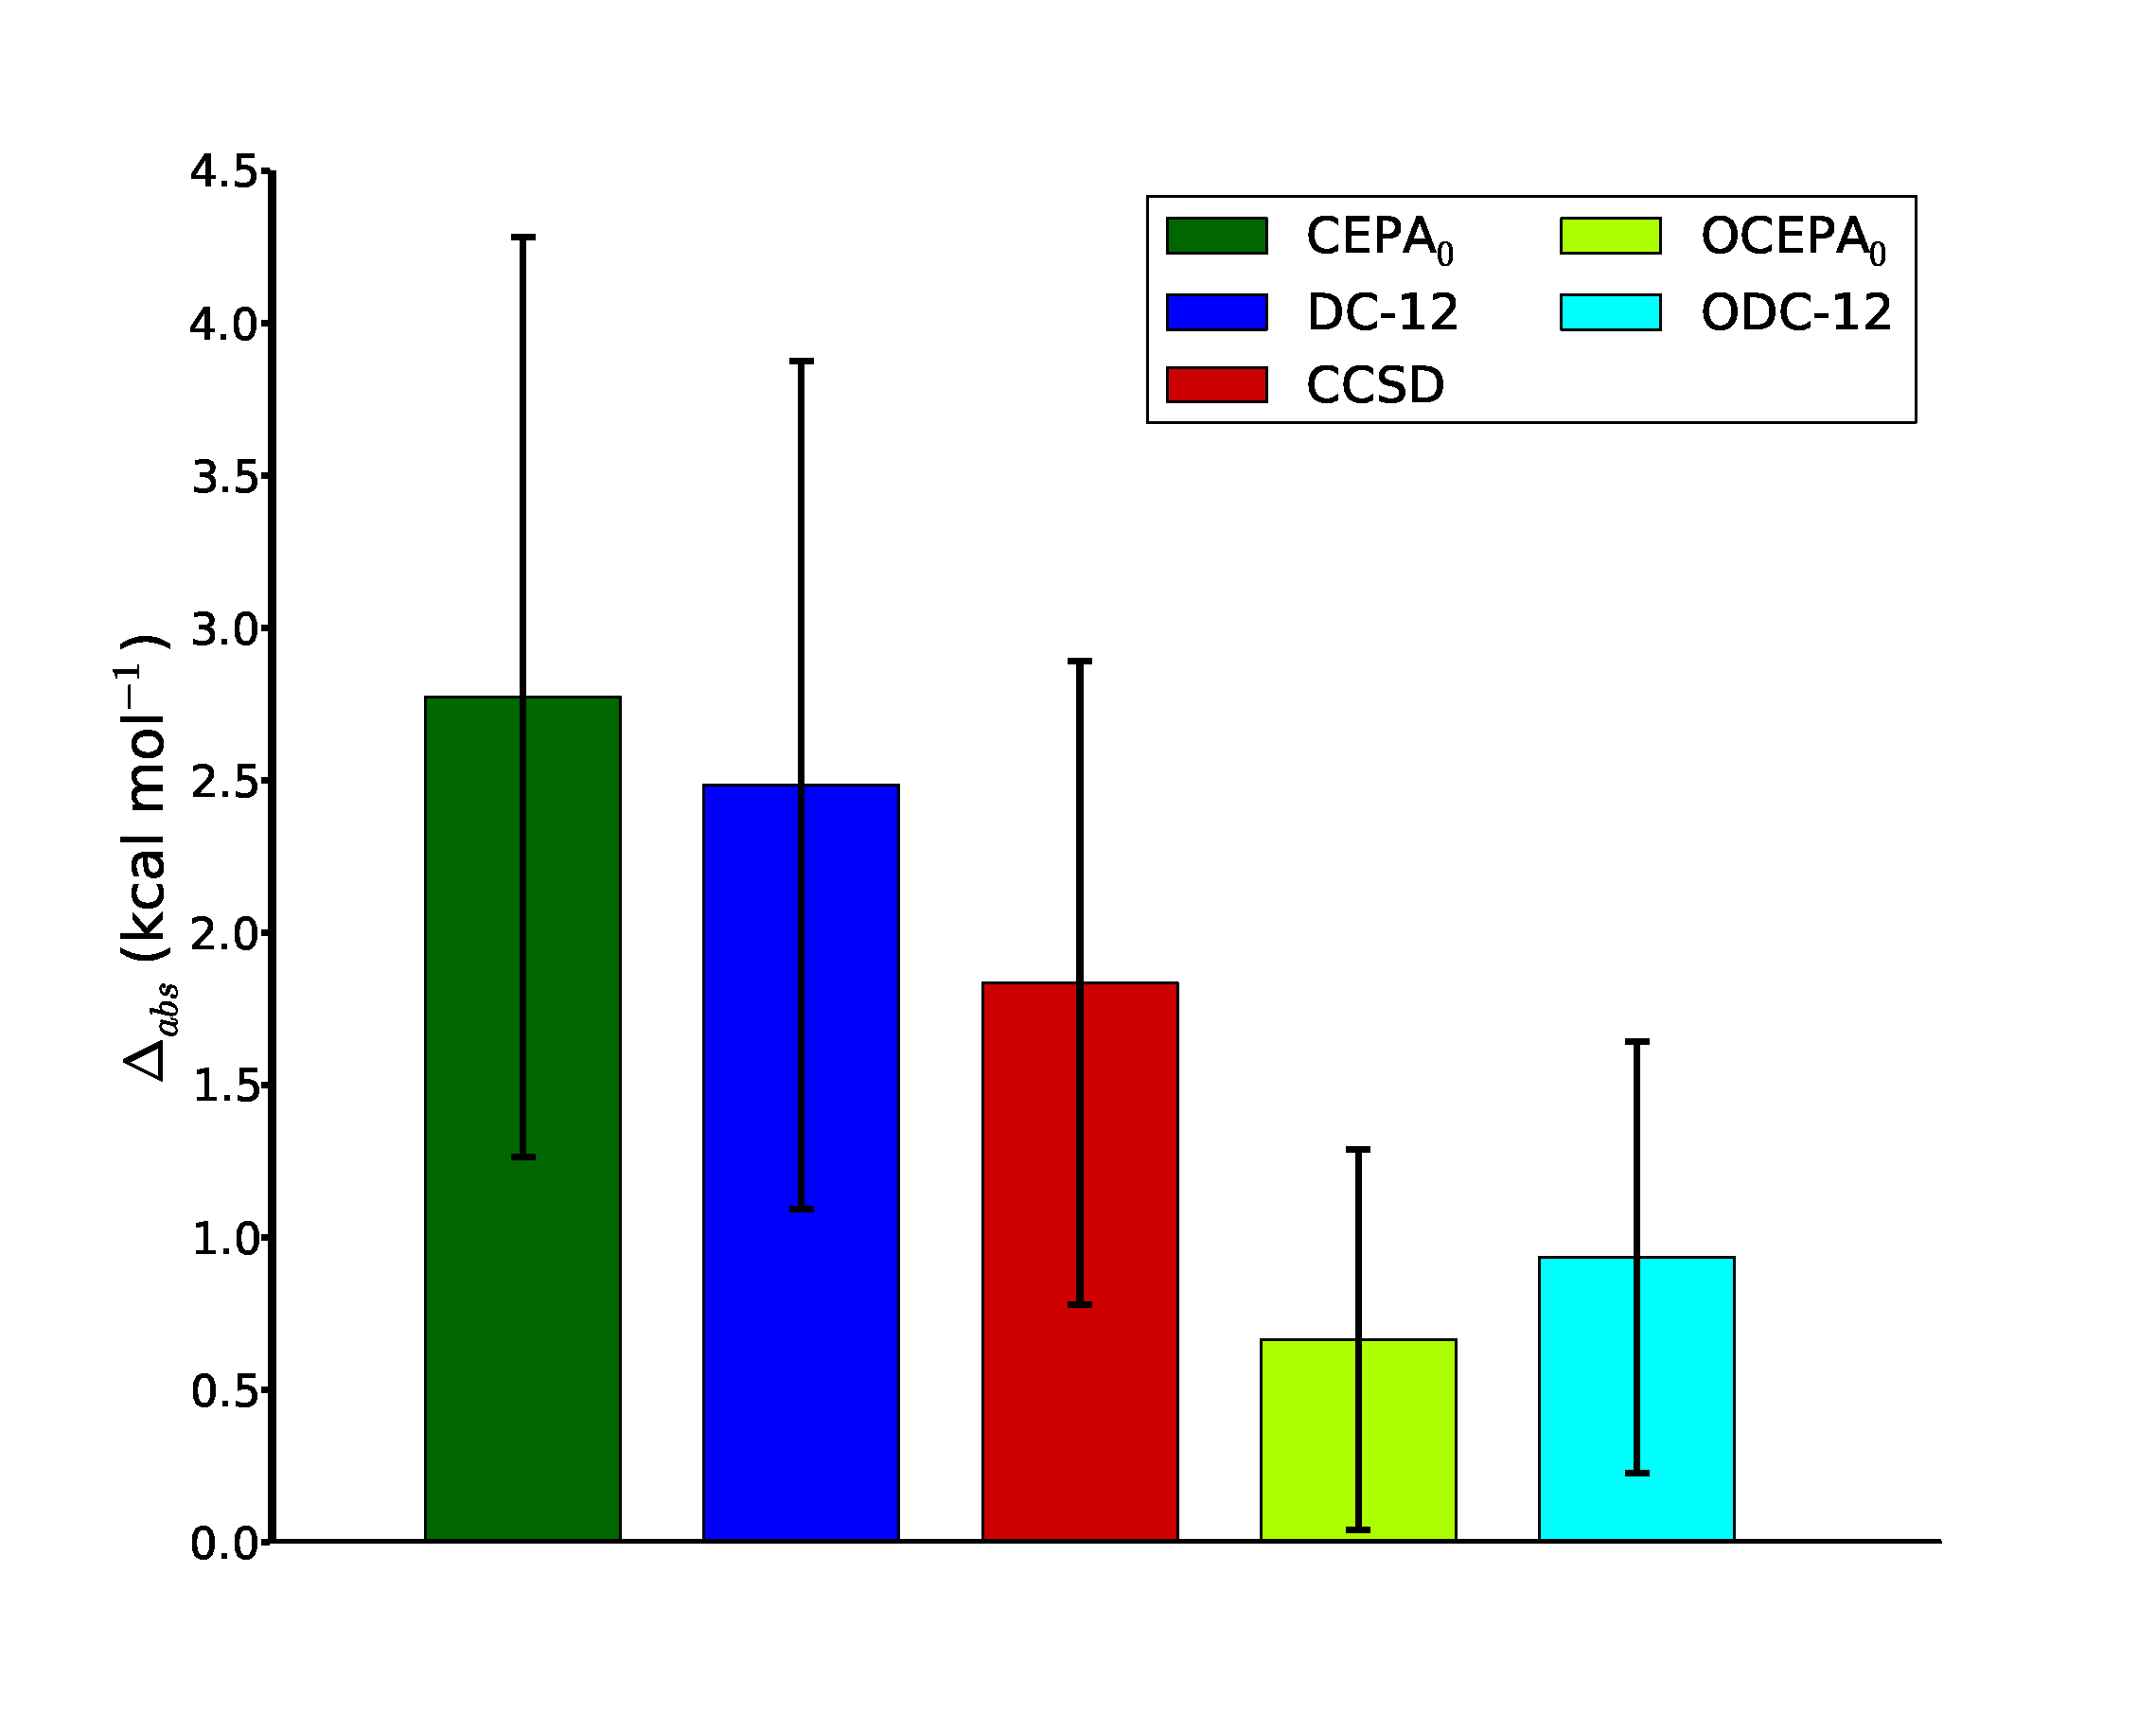
\includegraphics[width=0.8\textwidth]{figures/htbh.pdf}
    \captionof{figure}{%
        \label{htbh-f}
        Mean absolute deviations (\mae, \kcal) and the standard deviations
        from the mean signed error (\std, \kcal) of barrier heights for 18
        hydrogen-transfer reactions (\ce{R1 + R2H $\rightarrow$ R1H + R2},
        HTBH38 database) computed using five methods with the aug-cc-pVTZ
        basis set.
        The errors are relative to CCSD(T)/aug-cc-pVTZ reference values.
        The \mae value is represented as a height of each colored box, while
        the \std value is depicted as a radius of the black vertical bar.
        See \cref{htbh-t} for data on individual database members.
    }
}

We continue by assessing the performance of DCFT methods in predicting barrier
heights for 18 hydrogen-transfer reactions from the HTBH38
database:\cite{Zhao:2005p43}
\begin{equation}
    \ce{R1 + R2H -> [R1R2H]^* -> R1H + R2}
\end{equation}
These reactions\footnote{Reaction 19 in HTBH38, the cis-trans isomerization of
piperylene, is omitted in the present study.} involve molecules ($\mathrm{R_1}$
and $\mathrm{R_2}$) and transition states ($\mathrm{[R_1R_2H]^*}$) with
open-shell character, making their properties more sensitive to electron
correlation effects. 
We employ barrier heights computed at the CCSD(T)/aug-cc-pVTZ level of theory as
our reference rather than the values provided by Lynch\cite{MN-Database} in
order to effectively exclude basis-set incompleteness effects. We also omit the
DC-06 and ODC-06 methods, which encounter frequent convergence problems due to
the poor description of $N$-representability (see Supporting Information for
incomplete DC-06 results).

Mean absolute deviations (\mae) and standard deviations (\std) for the
hydrogen-transfer barrier heights are presented in \cref{htbh-t} and plotted in
\cref{htbh-f}.
The largest \mae values come from CEPA$_0$ and DC-12 (2.77 and 2.49~\kcal,
respectively).
Orbital optimization greatly improves the accuracy of these methods, resulting
in \mae values of just 0.67 and 0.94~\kcal for OCEPA$_0$ and ODC-12,
respectively.
The CCSD method shows intermediate performance with \mae = 1.84~\kcal.
A similar trend is observed for the \std values, with OCEPA$_0$ (0.62~\kcal) and
ODC-12 (0.71~\kcal) significantly improving upon CEPA$_0$ (1.51~\kcal), DC-12
(1.39~\kcal), and CCSD (1.06~\kcal).
In addition to \mae and \std, \cref{htbh-t} includes mean percent error (\rel)
values, which are commonly used to benchmark performance for reaction kinetics.
The smallest \rel values are 29\% and 40\% for OCEPA$_0$ and ODC-12,
respectively.

Turning to barrier heights for individual hydrogen-transfer reactions
(\cref{htbh-t}), the largest errors are observed for reactions 6 and 14, both
involving the OH radical, for which CEPA$_0$ and DC-12 give errors of $\sim$
5-6~\kcal.
The best results for these reactions are obtained from OCEPA$_0$, with errors
ranging from 0.51 to 1.18~\kcal.
The ODC-12 method tends to predict larger barrier heights than OCEPA$_0$,
yielding smaller errors only when OCEPA$_0$ underestimates the barrier heights.

\subsection{Radical Stabilization Energies}

\afterpage{%
    \clearpage
    \centering
    \begin{landscape}
        \vspace*{\fill}
        \captionof{table}{%
            \label{rse-t}
            Errors in radical stabilization energies (RSEs, \kcal) for 30
            open-shell doublet species (\ce{{}^.R}) comprising the RSE30
            database \cite{Soydas:2013p1452} computed using six methods with
            the cc-pCVTZ basis set.
            The errors are relative to CCSD(T) with an added quadruples
            correction ($\delta Q = E_\mathrm{CCSDT(Q)}-E_\mathrm{CCSD(T)}$)
            shown in the rightmost column in \kcal.
            The $\delta$Q correction was computed using the cc-pCVDZ basis
            set.  RSE is defined as the reaction enthalpy for the
            homodesmotic reaction \ce{{}^.CH3 + RH $\rightarrow$ CH4 +
            {}^.R}.
            To indicate the degree of spin-contamination in the UHF
            reference, the spin expectation values
            ($\langle\hat{\mathsf{S}}^2\rangle_{\text{SCF}}$) are also shown
            in units of $\hbar^2$.
            For each method the mean absolute deviations from
            CCSD(T)${+}\delta$Q (\mae, \kcal) and the standard deviations
            from the mean signed error (\std, \kcal) are also presented.
        }
        \vspace{1em}
        \renewcommand\arraystretch{0.6}
        \small
        \begin{tabular}{llrrrrrrrr}
            \hline
            \hline
            \ce{{}^.R} & \(\langle\hat{S}^2\rangle_\mathrm{SCF}\) &
            \(\Delta\)CEPA$_0$ & \(\Delta\)DC-12 & \(\Delta\)CCSD &
            \(\Delta\)OCEPA$_0$ & \(\Delta\)ODC-12 & \(\Delta\)CCSD(T) &
            CCSD(T){+}\(\delta\)Q
            \\
            \hline
            \ce{{}^.CH2NO2} &
            0.78  & 1.24 & 0.95 & 0.66 & 0.16 & 0.27 & 0.32 &
            -3.50 \\ 
            \ce{{}^.CH2OCHO} &
            0.76  & 1.16 & 1.12 & 0.63 & 0.40 & 0.48 & 0.10 &
            -4.84 \\
            \ce{{}^.CH2SCH3} &
            0.76  & 1.89 & 1.70 & 0.81 & 0.63 & 0.72 & 0.15 &
            -11.01 \\
            \ce{{}^.CF\bond{2}CH2} &
            0.94  & 6.12 & 3.71 & 0.96 & 0.42 & 0.64 & 0.46 &
            6.26 \\
            \ce{{}^.CH2CH2F} &
            0.76  & 0.30 & 0.27 & 0.13 & 0.08 & 0.10 & 0.04 &
            -1.53 \\
            \ce{{}^.CH2CHO} &
            0.93  & 5.01 & 2.86 & 0.32 & -0.16 & 0.02 & 0.46 &
            -10.11\\
            \ce{{}^.CH2CN} &
            0.94  & 6.36 & 3.52 & 0.65 & -0.02 & 0.21 & 0.46 &
            -8.66 \\
            \ce{{}^.CH2F} &
            0.76  & 1.03 & 1.00 & 0.52 & 0.55 & 0.57 & 0.06 &
            -4.22 \\
            \ce{{}^.CH2NH2} &
            0.76  & 1.28 & 1.18 & 0.59 & 0.50 & 0.52 & 0.06 &
            -12.06\\
            \ce{{}^.CH2NH3+} &
            0.76  & 0.16 & 0.10 & 0.08 & 0.06 & 0.03 & 0.02 &
            4.58 \\
            \ce{{}^.CH2NHOH} &
            0.77  & 1.76 & 1.57 & 0.78 & 0.58 & 0.64 & 0.15 &
            -8.81 \\
            \ce{{}^.CH2OH} &
            0.76  & 1.29 & 1.23 & 0.62 & 0.57 & 0.60 & 0.07 &
            -9.27 \\
            \ce{{}^.CH2PH3+} &
            0.76 & 0.21 & 0.14 & 0.01 & 0.01 & -0.02 & 0.05 &
            0.49 \\
            \ce{{}^.CH2SH2+} &
            0.77 & 0.41 & 0.30 & 0.12 & 0.11 & 0.08 & 0.06 &
            2.29 \\
            \ce{{}^.CH2SH} &
            0.76 & 1.60 & 1.43 & 0.68 & 0.57 & 0.63 & 0.12 &
            -9.68 \\
            \hline
        \end{tabular}
        \vspace*{\fill}
        \newpage
        \vspace*{\fill}
        \begin{tabular}{lllrrrrrrr}
            \hline
            \hline
            \ce{{}^.R} & \(\langle\hat{S}^2\rangle_\mathrm{SCF}\) &
            \(\Delta\)CEPA$_0$ & \(\Delta\)DC-12 & \(\Delta\)CCSD &
            \(\Delta\)OCEPA$_0$ & \(\Delta\)ODC-12 & \(\Delta\)CCSD(T) &
            CCSD(T){+}\(\delta\)Q
            \\
            \hline
            \ce{{}^.CH2C\bond{3}CH} &
            1.00  & 6.23 & 3.47 & 0.82 & -0.03 & 0.23 & 0.52 &
            -13.17\\
            \ce{{}^.CH2CH3} &
            0.76  & 0.30 & 0.26 & 0.11 & 0.08 & 0.10 & 0.03 &
            -3.36 \\
            \ce{{}^.CH2Cl} &
            0.77 & 1.13 & 1.02 & 0.50 & 0.48 & 0.51 & 0.09 &
            -5.67 \\
            \ce{{}^.CH2BH2} &
            0.76 & 0.17 & 0.17 & 0.05 & 0.03 & 0.04 & 0.05 &
            -11.66\\
            \ce{{}^.CHO} &
            0.77  & 2.26 & 2.24 & 1.48 & 1.55 & 1.56 & 0.20 &
            -17.61\\
            \ce{{}^.CH2PH2} &
            0.76 & 1.17 & 1.02 & 0.39 & 0.36 & 0.39 & 0.12 &
            -6.50 \\
            \ce{{}^.CHClF} &
            0.76  & 1.61 & 1.52 & 0.76 & 0.78 & 0.81 & 0.13 &
            -6.61 \\
            \ce{{}^.CHFCH3} &
            0.76 & 1.07 & 1.01 & 0.50 & 0.51 & 0.53 & 0.08 &
            -5.87 \\
            \ce{{}^.CH(OH)2} &
            0.76 & 1.30 & 1.22 & 0.60 & 0.60 & 0.61 & 0.08 &
            -6.67 \\
            \ce{{}^.CHCl2} &
            0.77 & 1.78 & 1.57 & 0.72 & 0.72 & 0.75 & 0.15 &
            -9.56 \\
            \ce{{}^.CHF2} &
            0.76 & 1.50 & 1.48 & 0.78 & 0.83 & 0.85 & 0.10 &
            -4.07 \\
            \ce{CH2\bond{2}C^.\bond{1}CN} &
            1.39 & 19.10 & 11.50 & 2.36 & -0.31 & 0.29 & 1.80 &
            1.98 \\
            \ce{{}^.C\bond{3}CH} &
            1.15 & 11.20 & 6.51 & 0.77 & -0.78 & -0.07 & 0.82 &
            26.25 \\
            \ce{{}^.CH\bond{2}CH2} &
            0.94 & 5.42 & 3.01 & 0.58 & 0.11 & 0.31 & 0.40 &
            5.49 \\
            \ce{{}^.CH2\bond{1}CH\bond{2}CH2} &
            0.97 & 4.98 & 3.17 & 0.51 & 0.11 & 0.31 & 0.48 &
            -17.53 \\
            \hline
            &&
            \mae: &
            2.97 & 2.01 & 0.62 & 0.40 & 0.43 & 0.25	&
            \\
            &&
            \std: &
            3.97 & 2.27 & 0.45 & 0.43 & 0.35 & 0.35	&
            \\
            \hline
            \hline
        \end{tabular}
        \vspace*{\fill}
    \end{landscape}
    \newpage
    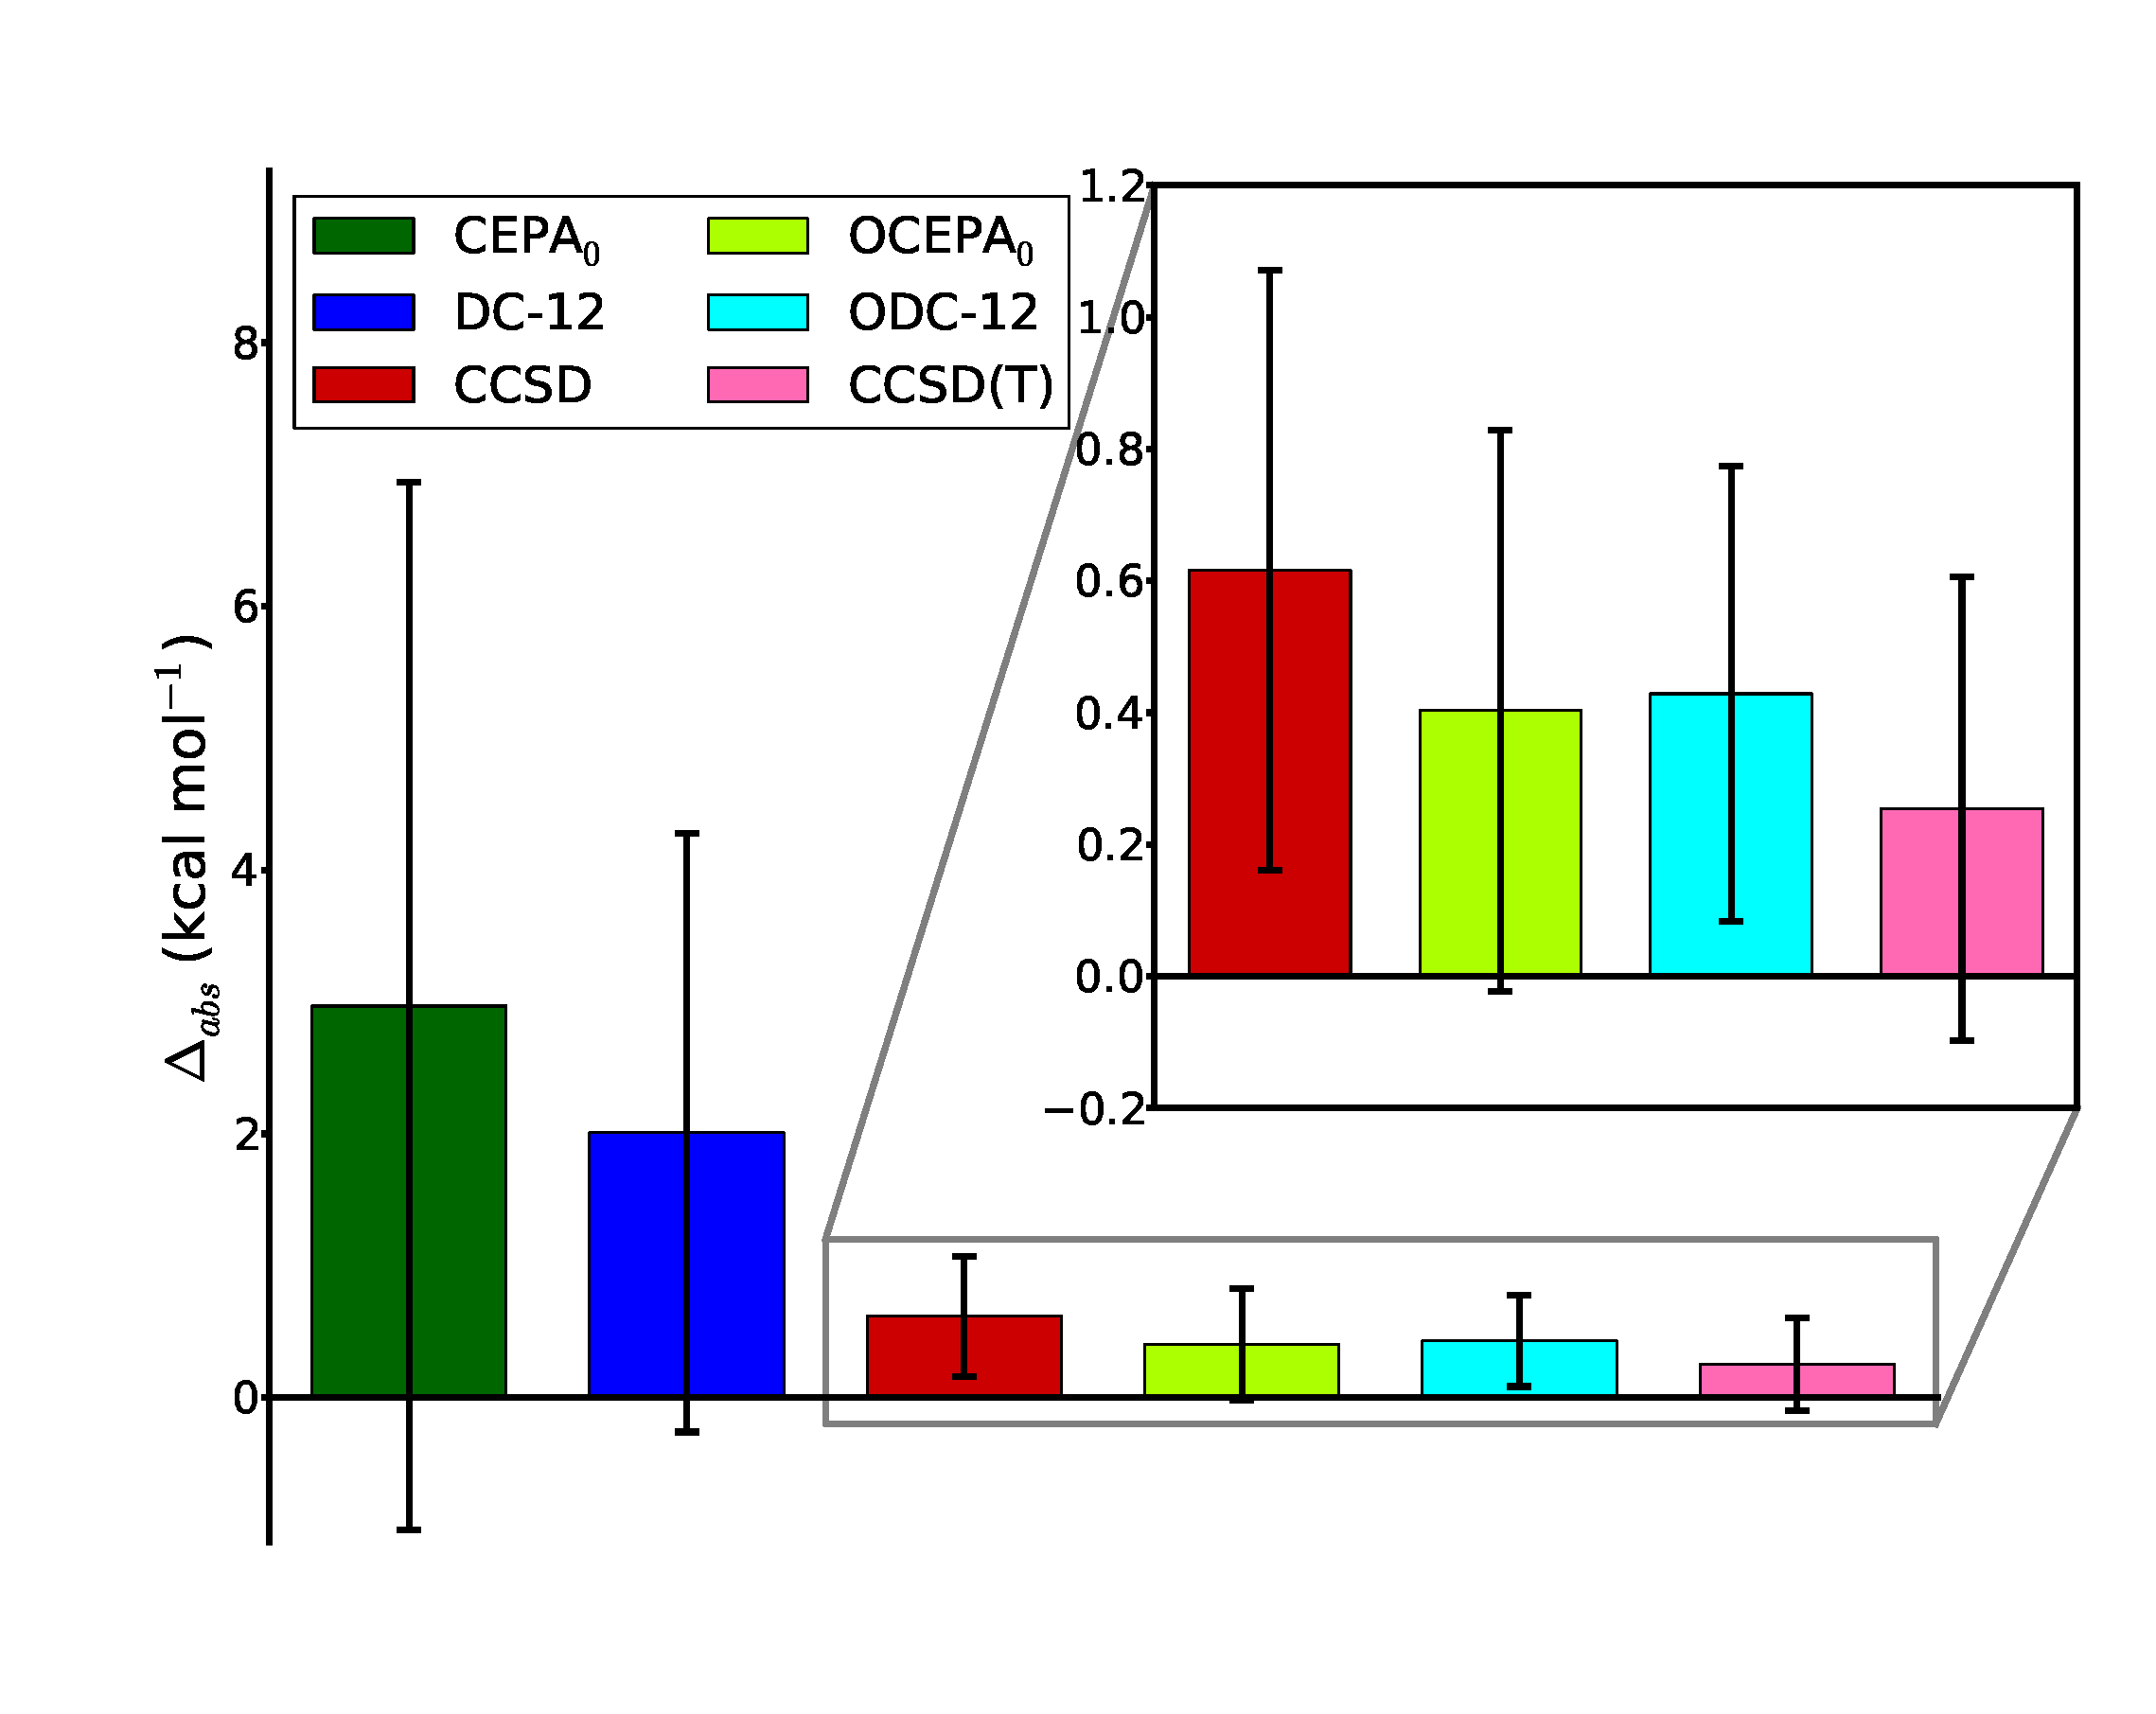
\includegraphics[width=0.8\textwidth]{figures/rse.pdf}
    \captionof{figure}{%
        \label{rse-f}
        Mean absolute deviations (\mae, \kcal) and the standard deviations
        from the mean signed error (\std, \kcal) of the radical
        stabilization energies (RSEs) for 30 open-shell doublet species
        (RSE30 database) computed using six methods with the cc-pCVTZ basis
        set.
        The errors are relative to CCSD(T) with an added quadruples
        correction ($\delta$Q  $= E_\mathrm{CCSDT(Q)}-E_\mathrm{CCSD(T)}$).
        The $\delta$Q correction was computed using the cc-pCVDZ basis set.
        RSE is defined as the reaction enthalpy for the homodesmotic
        reaction \ce{{}^.CH3 + RH $\rightarrow$ CH4 + {}^.R}.
        The \mae value is represented as a height of each colored box, while
        the \std value is depicted as a radius of the black vertical bar.
        See \cref{rse-t} for data on individual database members.
    }
}

In this section we study the performance of DCFT methods for predicting radical
stabilization energies (RSEs). An R-group's RSE is defined as the enthalpy of a
homodesmotic reaction
\begin{equation}
    \ce{%
        RH
        +
        {}^.CH3
        ->
        {}^.R
        +
        CH4
    }
\end{equation}
where exothermic (negative) values indicate that the radical \ce{{}^.R} is more
thermodynamically stable than \ce{{}^.CH3}.\cite{Zipse:2006p163}
For our benchmark we use the RSE30 dataset\cite{Soydas:2013p1452}, which
provides a diverse variety of \ce{{}^.R} species (listed in \cref{rse-t}).
Since the performance of CCSD(T) is known to deteriorate for strongly
spin-contaminated UHF
references,\cite{Byrd:2001p9736,Beran:2003p2488,Lochan:2007p164101,Kurlancheek:2009p1223,Bozkaya:2011p224103}
we augment CCSD(T) energies with a quadruples correction ($\Delta$Q  =
$E_\mathrm{CCSDT(Q)}-E_\mathrm{CCSD(T)}$) and use these as our benchmark.
CBS-extrapolated CCSD(T) reference values have been published for this
dataset,\cite{Soydas:2014p1073} but we use CCSD(T) values computed with the
cc-pCVTZ basis set to avoid basis-set incompleteness effects. 
The $\delta$Q correction was evaluated using the cc-pCVDZ basis set. 
As in the previous Section, DC-06 and ODC-06 computations cannot be converged
for all database members and are omitted in the analysis below (see Supporting
Information for incomplete DC-06 and ODC-06 data).


The relative performance of the DCFT, CEPA, and CC methods for the RSE30 dataset
is shown in \cref{rse-f}.
The effect of orbital-optimization on accuracy is now even more pronounced,
reducing the large \mae errors of CEPA$_0$ (2.97~\kcal) and DC-12 (2.01~\kcal)
to 0.40 and 0.43~\kcal for OCEPA$_0$ and ODC-12, respectively. CCSD has a
slightly larger \mae value (0.62~\kcal), while CCSD(T) has the smallest overall
\mae (0.25~\kcal).
Both CEPA$_0$ and DC-12 show large standard deviations again (3.97 and
2.27~\kcal, respectively).
For OCEPA$_0$, the standard deviation (0.43~\kcal) is similar to that of CCSD
(0.45~\kcal). ODC-12 and CCSD(T) exhibit the most consistent performance with
the same \std value of 0.35~\kcal.

Deviations from CCSD(T){+}\(\delta\)Q for individual RSEs predicted by each
method are tabulated in \cref{rse-t}.
In addition, \cref{rse-t} includes expectation values of the square-norm spin
operator computed for the UHF wavefunction of \ce{{}^.R}
($\langle\hat{S}^2\rangle_\mathrm{SCF}$).
The largest errors in computed RSEs were obtained for \ce{{}^.R} species with
\(
    \langle\hat{S}^2\rangle_\mathrm{SCF}
    >
    0.9\
    \hbar^2
\)
(radicals 4, 6, 7, 16, and 27-30 in \cref{rse-t}).
For these systems, the average CEPA$_0$ and DC-12 errors are 8.05 and
4.72~\kcal, and the average CCSD(T) error is 0.68~\kcal.
OCEPA$_0$ and ODC-12 offer remarkably better performance for this subset, with
average errors of 0.24~\kcal and 0.26~\kcal.


\afterpage{%
    \clearpage
    \centering
    \begin{landscape}
        \vspace*{\fill}
        \captionof{table}{%
            \label{ip-t}
            Errors in adiabatic ionization energies (AIEs, \eV) for 10 di-
            and triatomic molecules computed using six methods with the
            cc-pCVQZ basis set.
            The errors are relative to experimental values
            (\(\mathrm{IE}_\mathrm{ref}\), \eV) from
            Ref.~\citenum{Lias:1988p1}, unless noted otherwise.
            For all AIEs the harmonic zero-point vibrational energy
            corrections were included.
            For each method the mean absolute deviations from
            \(\mathrm{IE}_\mathrm{ref}\) (\mae, \eV) and the standard
            deviations from the mean signed error (\std, \eV) are also
            shown.
        }
        \vspace{1em}
        \renewcommand\arraystretch{0.6}
        \small
        \begin{threeparttable}
            \begin{tabular}{ccrrrrrrc}
                \hline
                \hline
                Molecule & Transition &
                $\Delta$CEPA$_0$ &
                $\Delta$DC-12 &
                $\Delta$CCSD &
                $\Delta$OCEPA$_0$ &
                $\Delta$ODC-12 &
                $\Delta$CCSD(T) &
                $\mathrm{IE}_\mathrm{ref}$
                \\
                \hline
                \ce{N2} &
                \(\termsymbol{{}^1\Sigma_g^+}\rightarrow\termsymbol{{}^2\Sigma_g^+}\) &
                0.08 & 0.17 & 0.12 &-0.05 & 0.07 &-0.03 &
                15.581  $\pm$ 0.008 \tnote{a} \\
                \ce{O2} &
                \(\termsymbol{{}^3\Sigma_g^-}\rightarrow\termsymbol{{}^2\Pi_g}\) &
                -0.11 &-0.03 & 0.04 &-0.09 &-0.02 &-0.04 &
                12.0697 $\pm$ 0.0002 \\
                \ce{F2} &
                \(\termsymbol{{}^1\Sigma_g^+}\rightarrow\termsymbol{{}^2\Pi_g}\) &
                0.06 & 0.06 & 0.04 & 0.08 & 0.01 &-0.03	&
                15.697 $\pm$ 0.003 \\
                \ce{NO} &
                \(\termsymbol{{}^2\Pi}\rightarrow\termsymbol{{}^1\Sigma^+}\) &
                -0.15 &-0.05 &-0.05 &-0.05 &-0.02 &-0.09 &
                9.26438 $\pm$ 0.00005 \\
                \ce{OF} &
                \(\termsymbol{{}^2\Pi}\rightarrow\termsymbol{{}^3\Sigma^-}\) &
                0.11 & 0.12 &-0.10 &-0.03 &-0.02 &-0.11	&
                12.77 $\pm$ 0.01 \tnote{b} \\
                \ce{HNC} &
                \(\termsymbol{{}^1\Sigma_g^+}\rightarrow\termsymbol{{}^2\Sigma^+}\) &
                0.27 & 0.14 &-0.12 &-0.14 &-0.08 &-0.04	&
                12.04 $\pm$ 0.01 \tnote{c} \\
                \ce{HOF} &
                \(\termsymbol{{}^1A'}\rightarrow\termsymbol{{}^2A''}\) &
                0.20 & 0.17 &-0.10 &-0.03 &-0.04 &-0.07	&
                12.71 $\pm$ 0.01 \\
                \ce{FNO} &
                \(\termsymbol{{}^1A'}\rightarrow\termsymbol{{}^2A''}\) &
                0.51 & 0.10 &-0.02 &-0.02 &-0.00 & 0.04	&
                12.63 $\pm$ 0.03 \\
                \ce{F2N} &
                \(\termsymbol{{}^2B_1}\rightarrow\termsymbol{{}^1A_1}\) &
                0.07 & 0.10 & 0.07 & 0.01 & 0.03 &-0.08	&
                11.63$\pm$ 0.01 \\
                \ce{F2O} &
                \(\termsymbol{{}^1A_1}\rightarrow\termsymbol{{}^2B_1}\) &
                0.49 & 0.37 &-0.01 & 0.05 & 0.04 &-0.04	&
                13.11 $\pm$ 0.01 \\
                \hline
                & \mae: & 0.21 & 0.13 & 0.06 & 0.05 & 0.03 & 0.06 & \\
                & \std: & 0.22 & 0.12 & 0.08 & 0.06 & 0.04 & 0.04 & \\
                \hline
                \hline
            \end{tabular}
            \begin{tablenotes}
                \item[a]
                    Reference \citenum{Trickl:1989p6006}.
                \item[b]
                    Reference \citenum{Zhang:1994p377}.
                \item[c]
                    Reference \citenum{Hansel:1998p1748}.
            \end{tablenotes}
        \end{threeparttable}
        \vspace*{\fill}
    \end{landscape}
    \newpage
	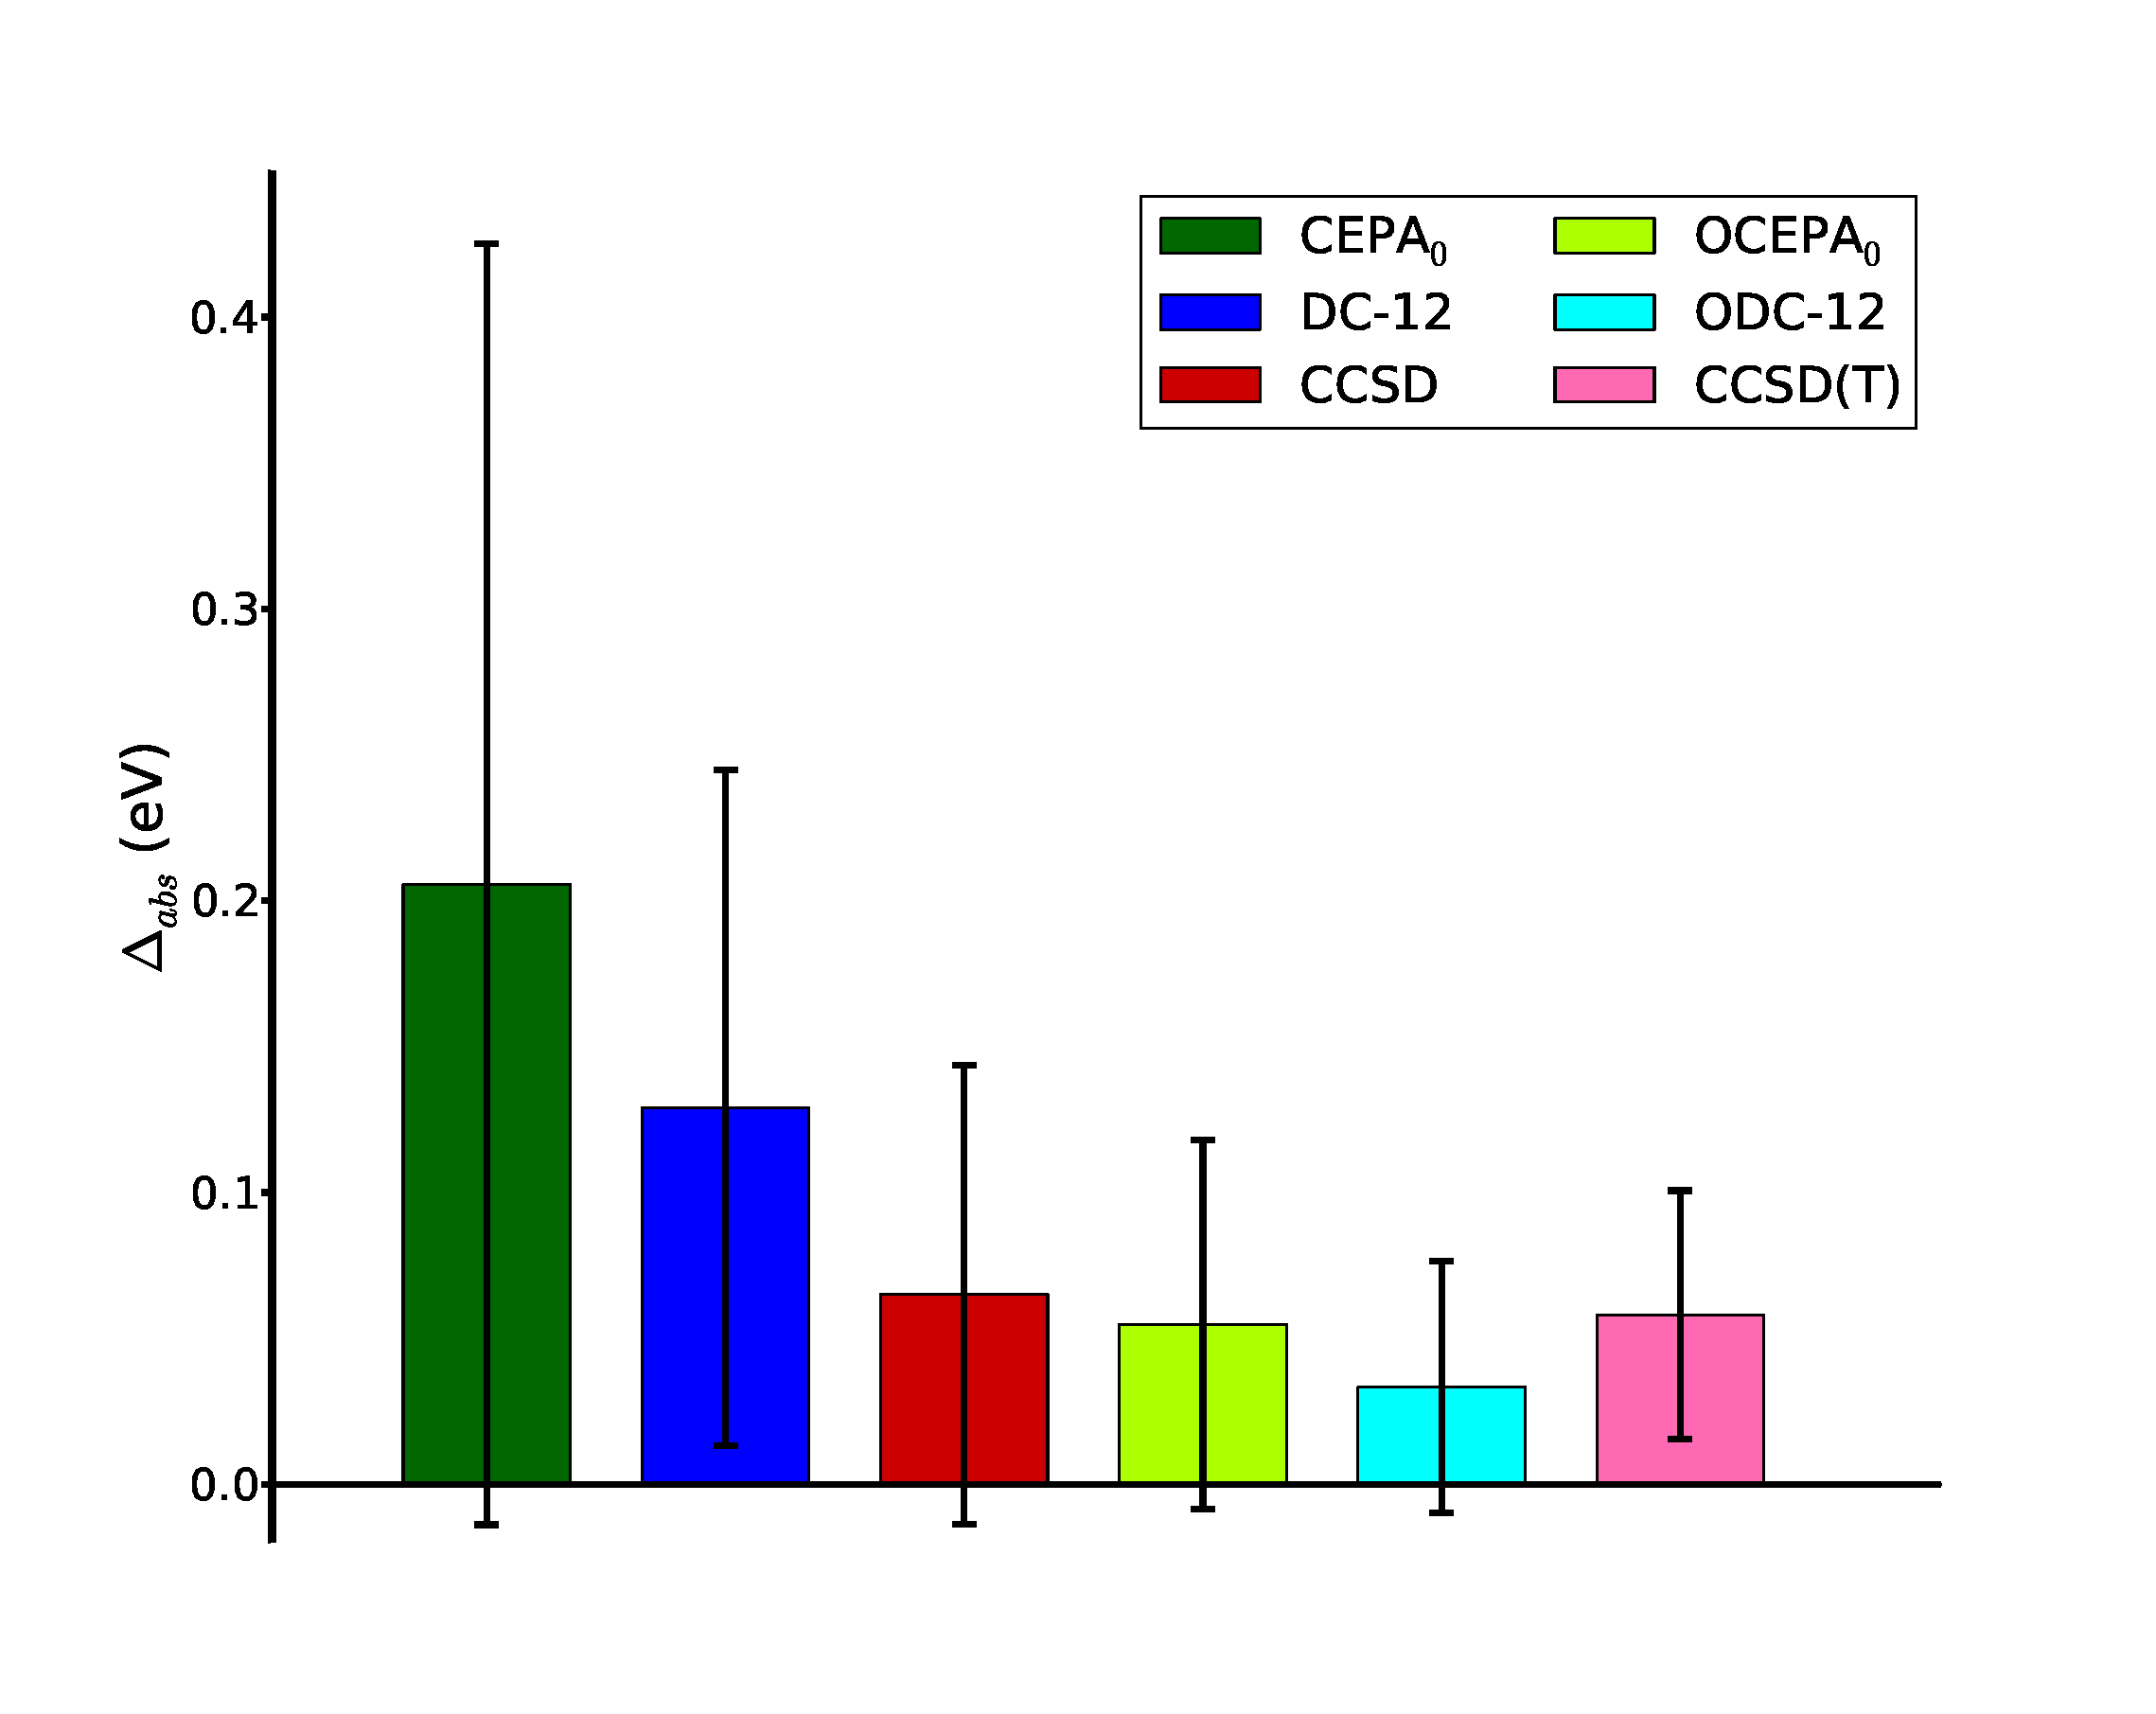
\includegraphics[width=0.8\textwidth]{figures/ip.pdf}
    \captionof{figure}{%
        \label{ip-f}
        Mean absolute deviations (\mae, \eV) and the standard deviations from
        the mean signed error (\std, \eV) of adiabatic ionization energies for
        10 di- and triatomic molecules computed using six methods with the
        cc-pCVQZ basis set.
        The errors are relative to experimental
        values.\cite{Lias:1988p1,Trickl:1989p6006,Zhang:1994p377,Hansel:1998p1748}
        The \mae value is represented as a height of each colored box, while the
        \std value is depicted as a radius of the black vertical bar.
        See \cref{ip-t} for data on individual molecules.
	}
}

\subsection{Adiabatic Ionization Energies in Electron-Dense Molecules}

We conclude the assessment of DCFT methods for the description of thermodynamic
properties by computing adiabatic ionization energies (AIEs) for a set of 10 di-
and triatomic electron-dense molecules (\cref{ip-t}), i.e.\ those that
are composed of elements with small atomic radius, high electron affinity, and
high electronegativity (N, O, F), in order to increase the magnitude of electron
correlation effects.
We use experimentally measured ionization energies reported to high precision
($\sim$0.01~\eV)\cite{Lias:1988p1,Trickl:1989p6006,Zhang:1994p377,Hansel:1998p1748}
as reference values for our benchmark (\(\mathrm{IE}_\mathrm{ref}\),
\cref{ip-t}).
The AIEs were computed using the cc-pCVQZ basis set, with harmonic ZPVE
corrections applied to each neutral and cationic system.

The \mae and \std values for our computed AIEs relative to experiment are
plotted in \cref{ip-f}.
Of the six methods, CEPA$_0$ and DC-12 exhibit the largest \mae values (0.21 and
0.13~\eV, respectively).
The closest agreement with experiment is given by ODC-12, with \mae = 0.03~\eV.
OCEPA$_0$, CCSD, and CCSD(T) show somewhat poorer performance (\mae = 0.05, 0.06
and 0.06~\eV, respectively). 
The \std for ODC-12 matches that of CCSD(T) (0.04~\eV).
For the other methods, the \std values decrease in the order CEPA$_0$ (0.22~\eV)
$>$ DC-12 (0.12) $>$ CCSD (0.08) $>$ OCEPA$_0$ (0.06).

Individual errors for each system are shown in \cref{ip-t}.
Both DC-12 and CEPA$_0$ exhibit large deviations for $\mathrm{F_2O}$ (0.49 and
0.37~\eV), and CEPA$_0$ also gives a large error for FNO (0.51~\eV) which is the
maximum error for this dataset.
Both DC-12 and CEPA$_0$ give errors exceeding 0.1~\eV for seven of the ten
systems, whereas CCSD exhibits errors in excess of 0.1~\eV for only three
systems (OF, HNC, and HOF).
CCSD(T) has only one such error (0.11~\eV for OF), as does OCEPA$_0$ (0.14~\eV
for HNC).
ODC-12 does the best of the methods considered, with a maximum error of
0.08~\eV, found for the AIE of HNC.


\begin{figure}
	\centering
	\caption{%
        \label{bh-f}
        Error in the total energy (\mhartree), relative to full CI, as a
        function of B--H internuclear separation (\AA) computed using six
        methods with the DZP basis set.
        The full CI reference is depicted with a horizontal dotted line.
        The dashed vertical line indicates the full CI equilibrium bond
        distance.
	}
	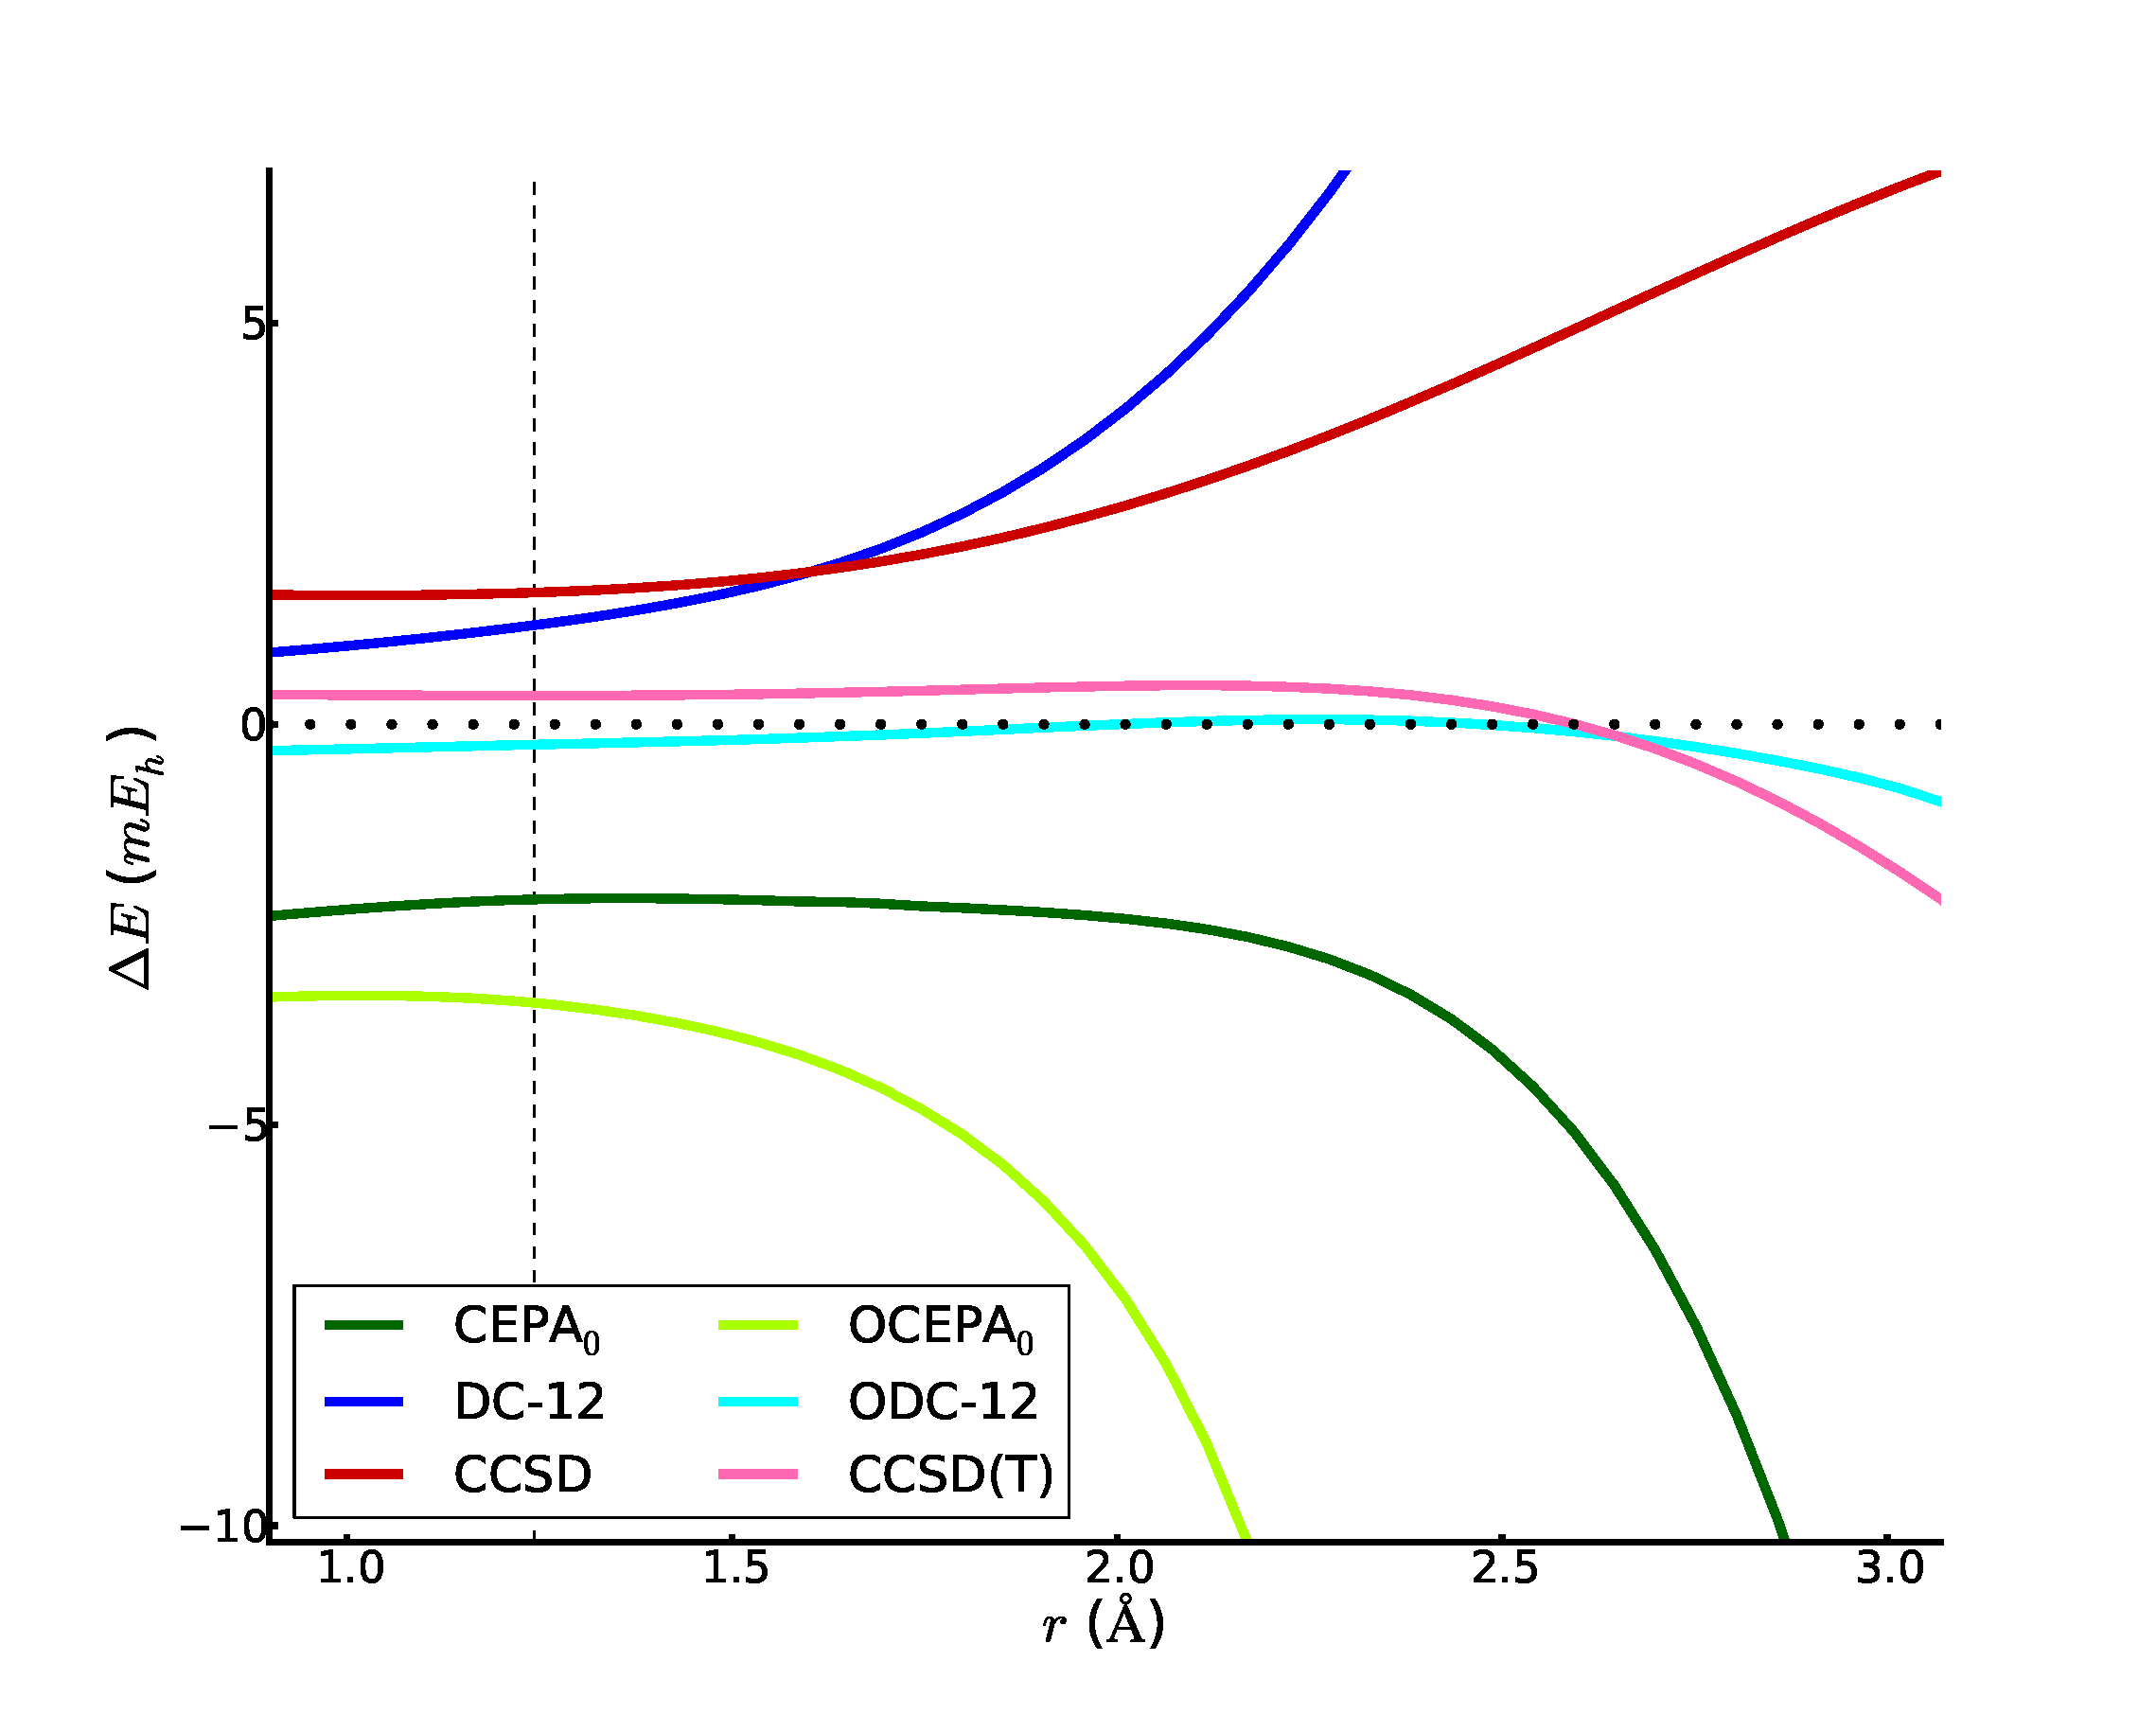
\includegraphics[width=0.8\textwidth]{figures/bh.pdf}
\end{figure}

\begin{figure}
	\centering
	\caption{%
        \label{hf-f}
        Error in the total energy (\mhartree), relative to full CI, as a
        function of H--F internuclear separation (\AA) computed using six
        methods with the DZP basis set.
        The full CI reference is depicted with a horizontal dotted line.
        The dashed vertical line indicates the full CI equilibrium bond
        distance.
	}
	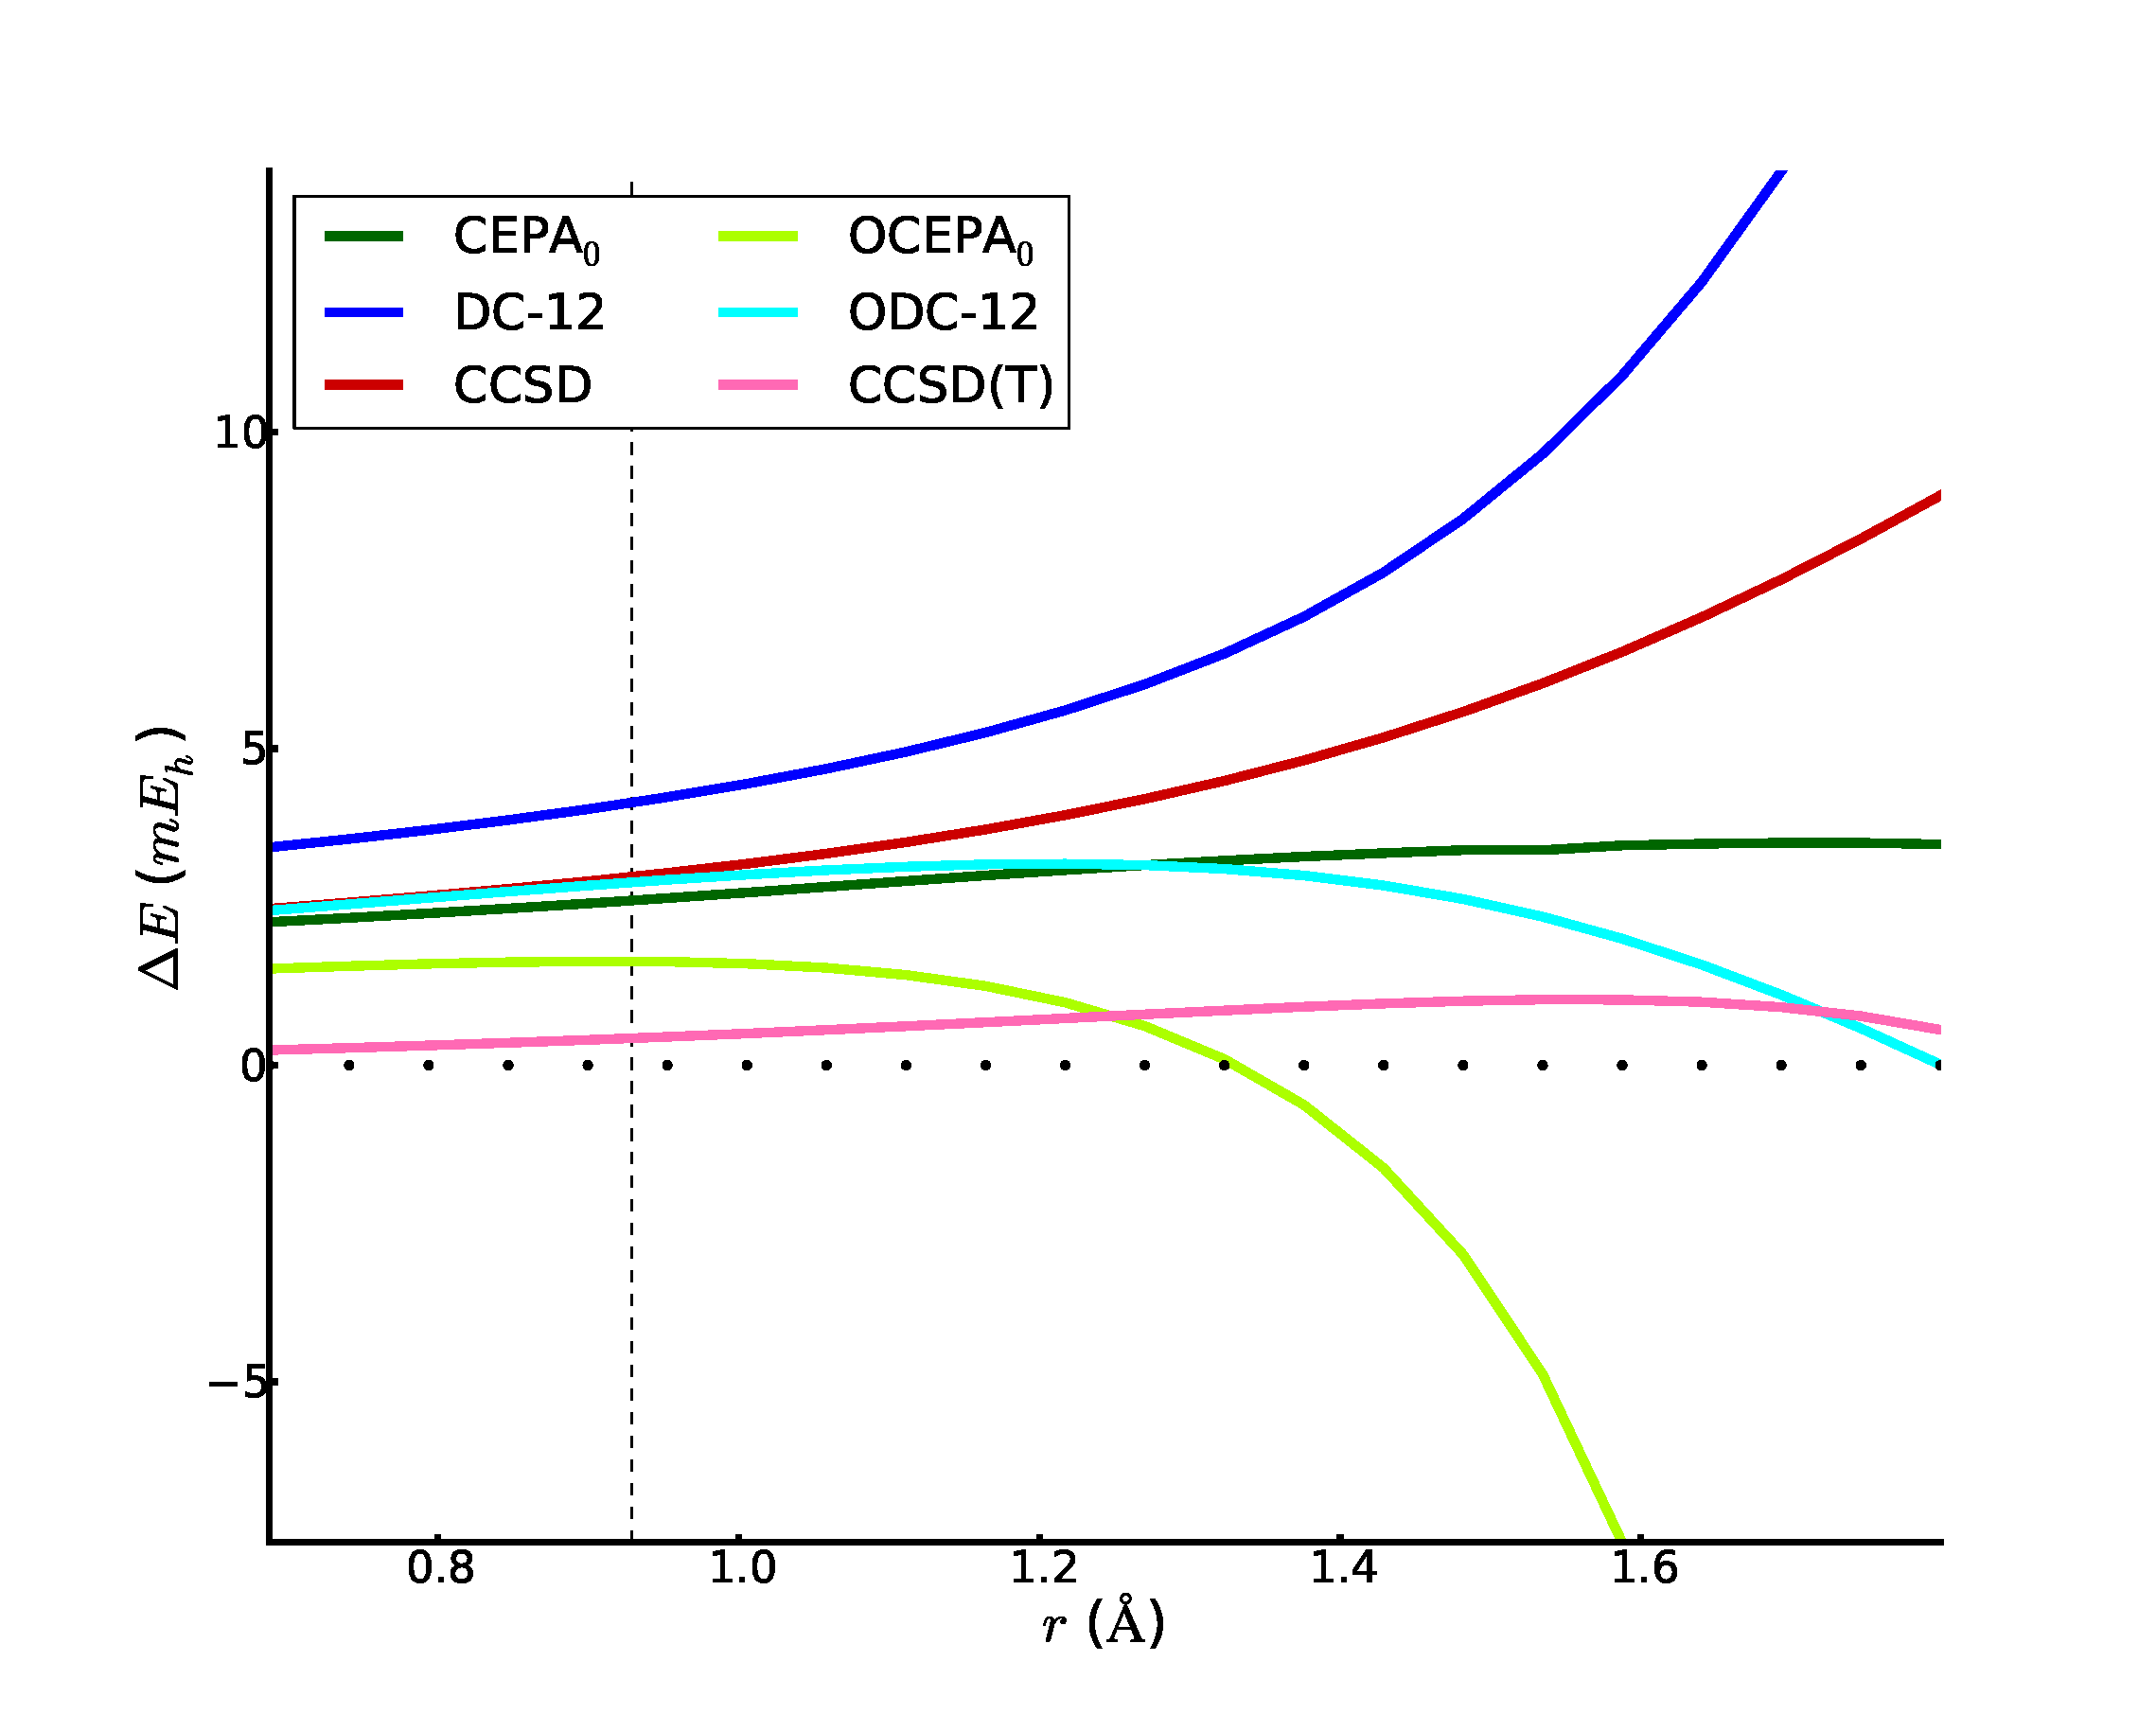
\includegraphics[width=0.8\textwidth]{figures/hf.pdf}
\end{figure}

\begin{figure}
	\centering
	\caption{%
        \label{beo-f}
        Error in the total energy (\mhartree), relative to full CI, as a
        function of Be--O internuclear separation (\AA) computed using six
        methods with the 6-31G basis set.
        The full CI reference is depicted with a horizontal dotted line.
        The dashed vertical line indicates the full CI equilibrium bond
        distance.
	}
	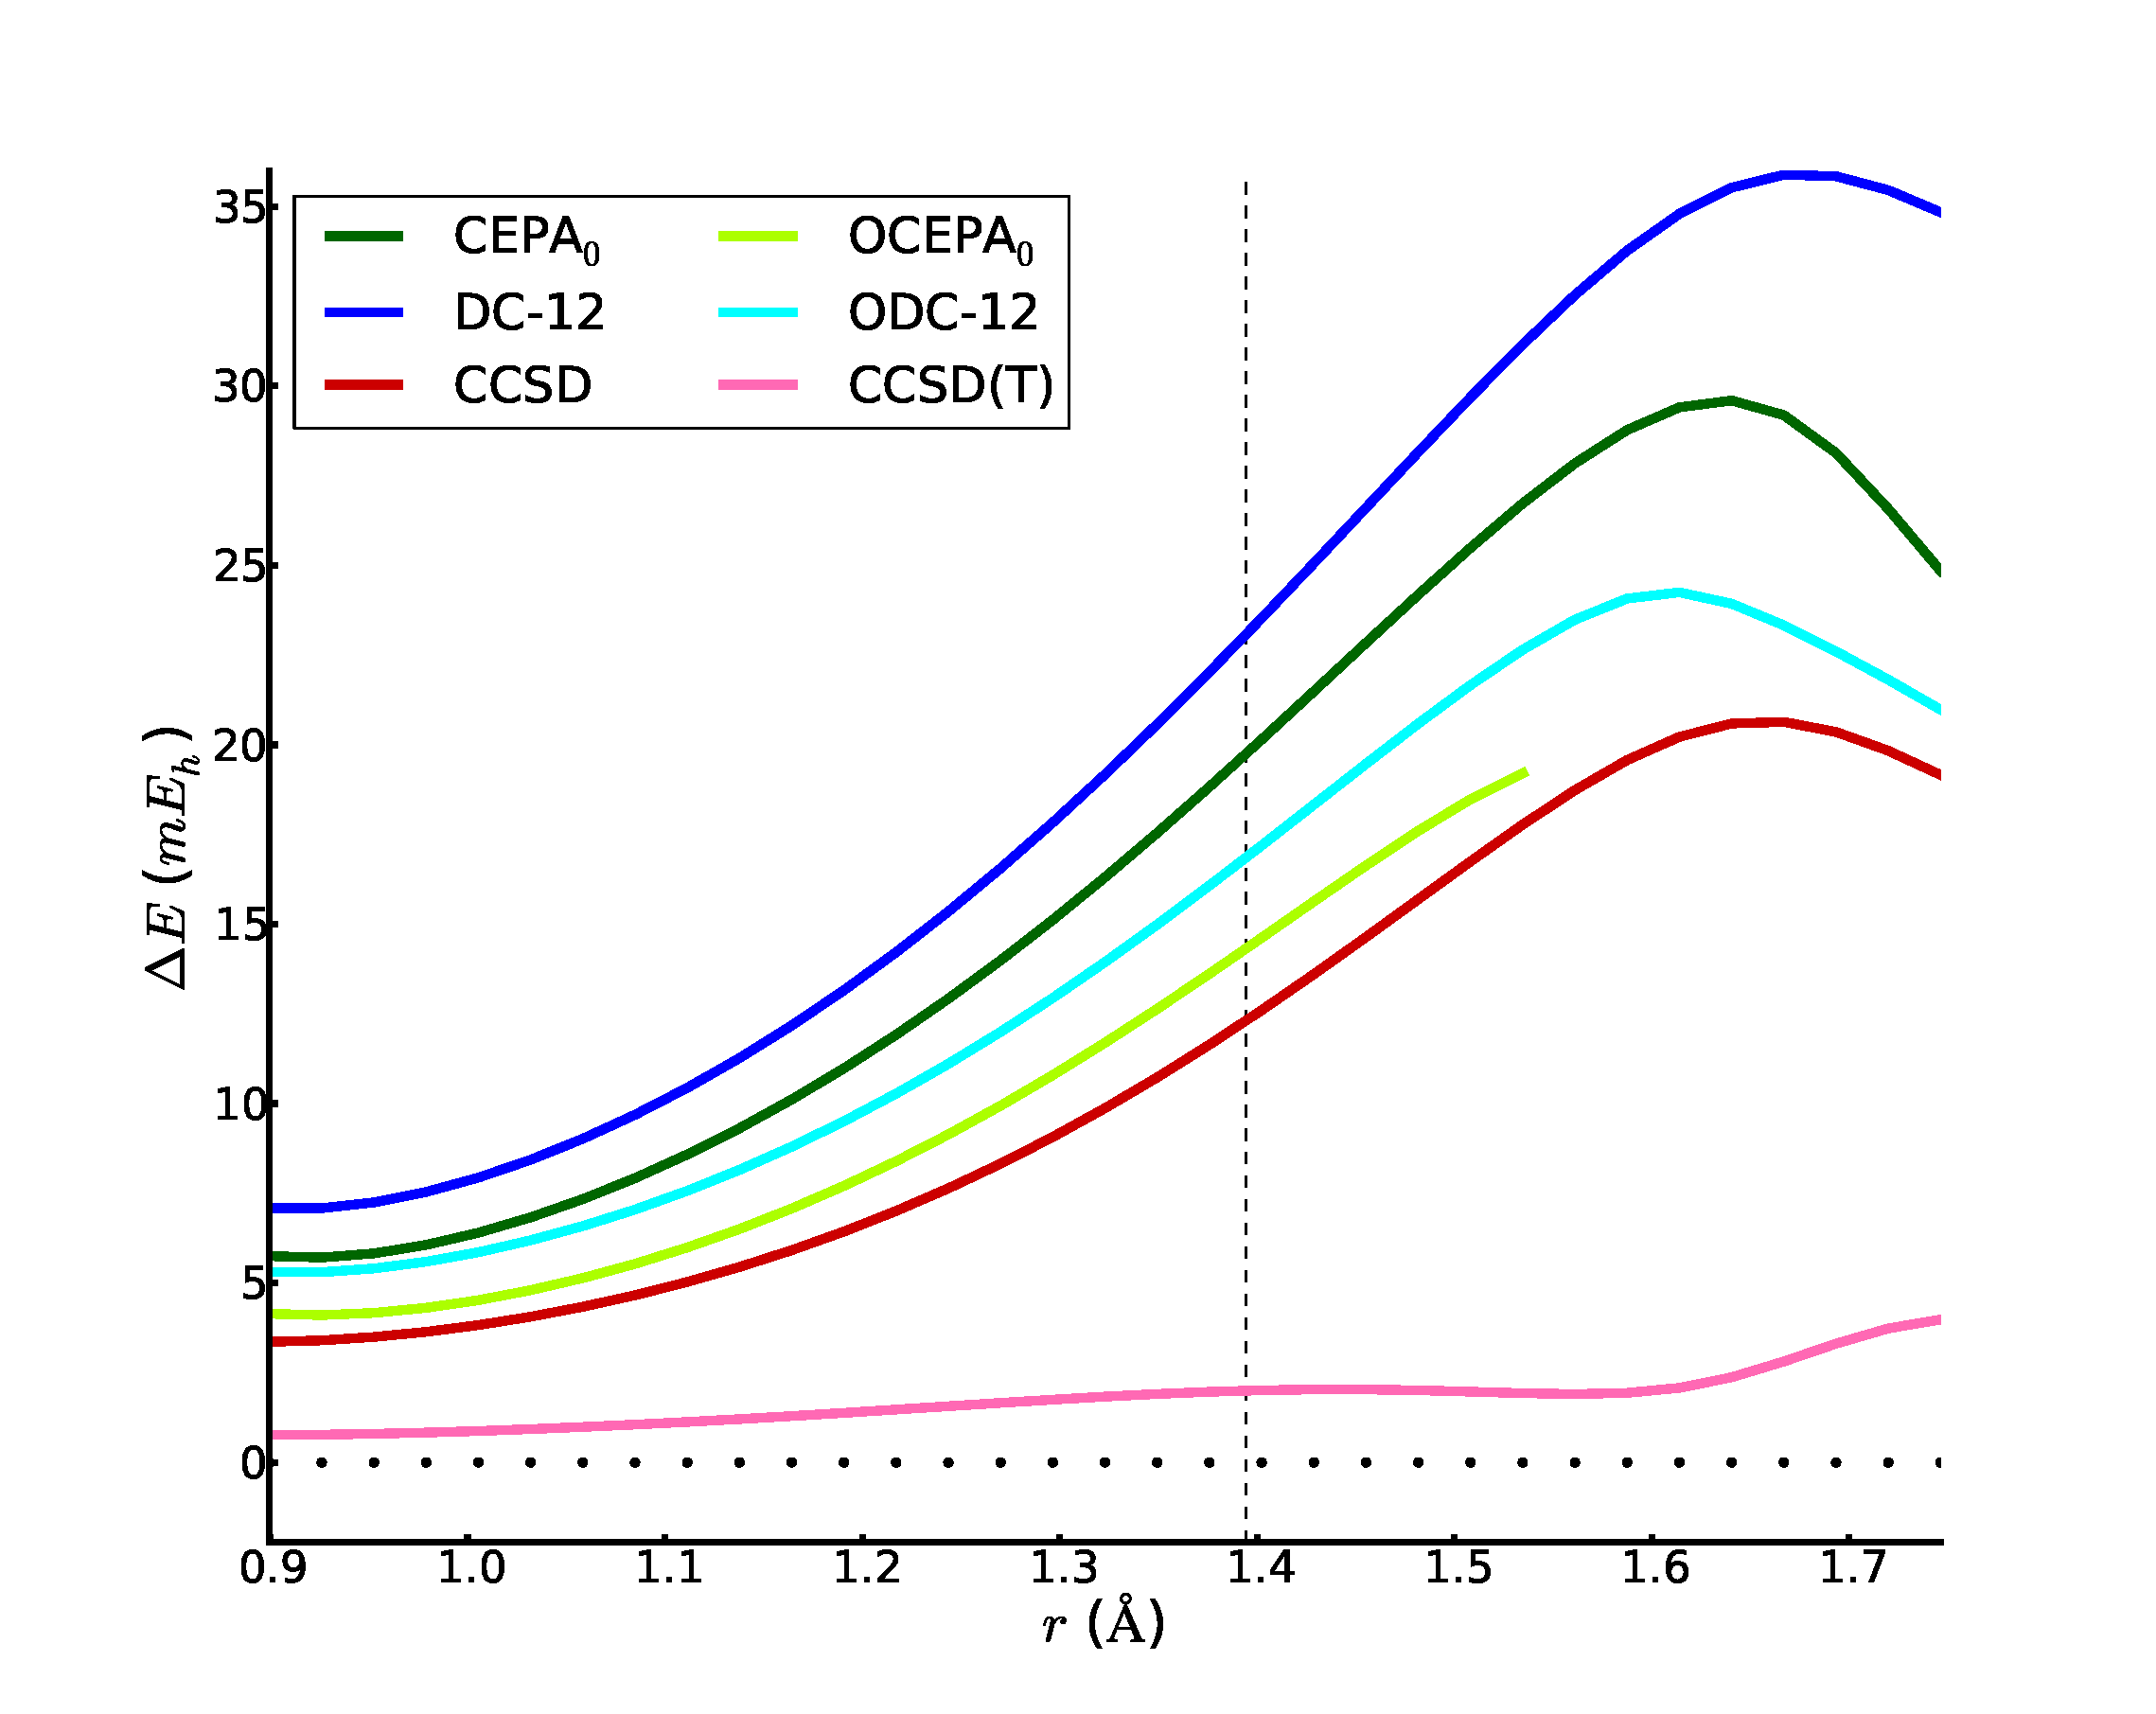
\includegraphics[width=0.8\textwidth]{figures/beo.pdf}
\end{figure}

\begin{figure}
	\centering
	\caption{%
        \label{n2-f}
        Error in the total energy (\mhartree), relative to full CI, as a
        function of N--N internuclear separation (\AA) computed using six
        methods with the 6-31G basis set.
        The full CI reference is depicted with a horizontal dotted line.
        The dashed vertical line indicates the full CI equilibrium bond
        distance.
	}
	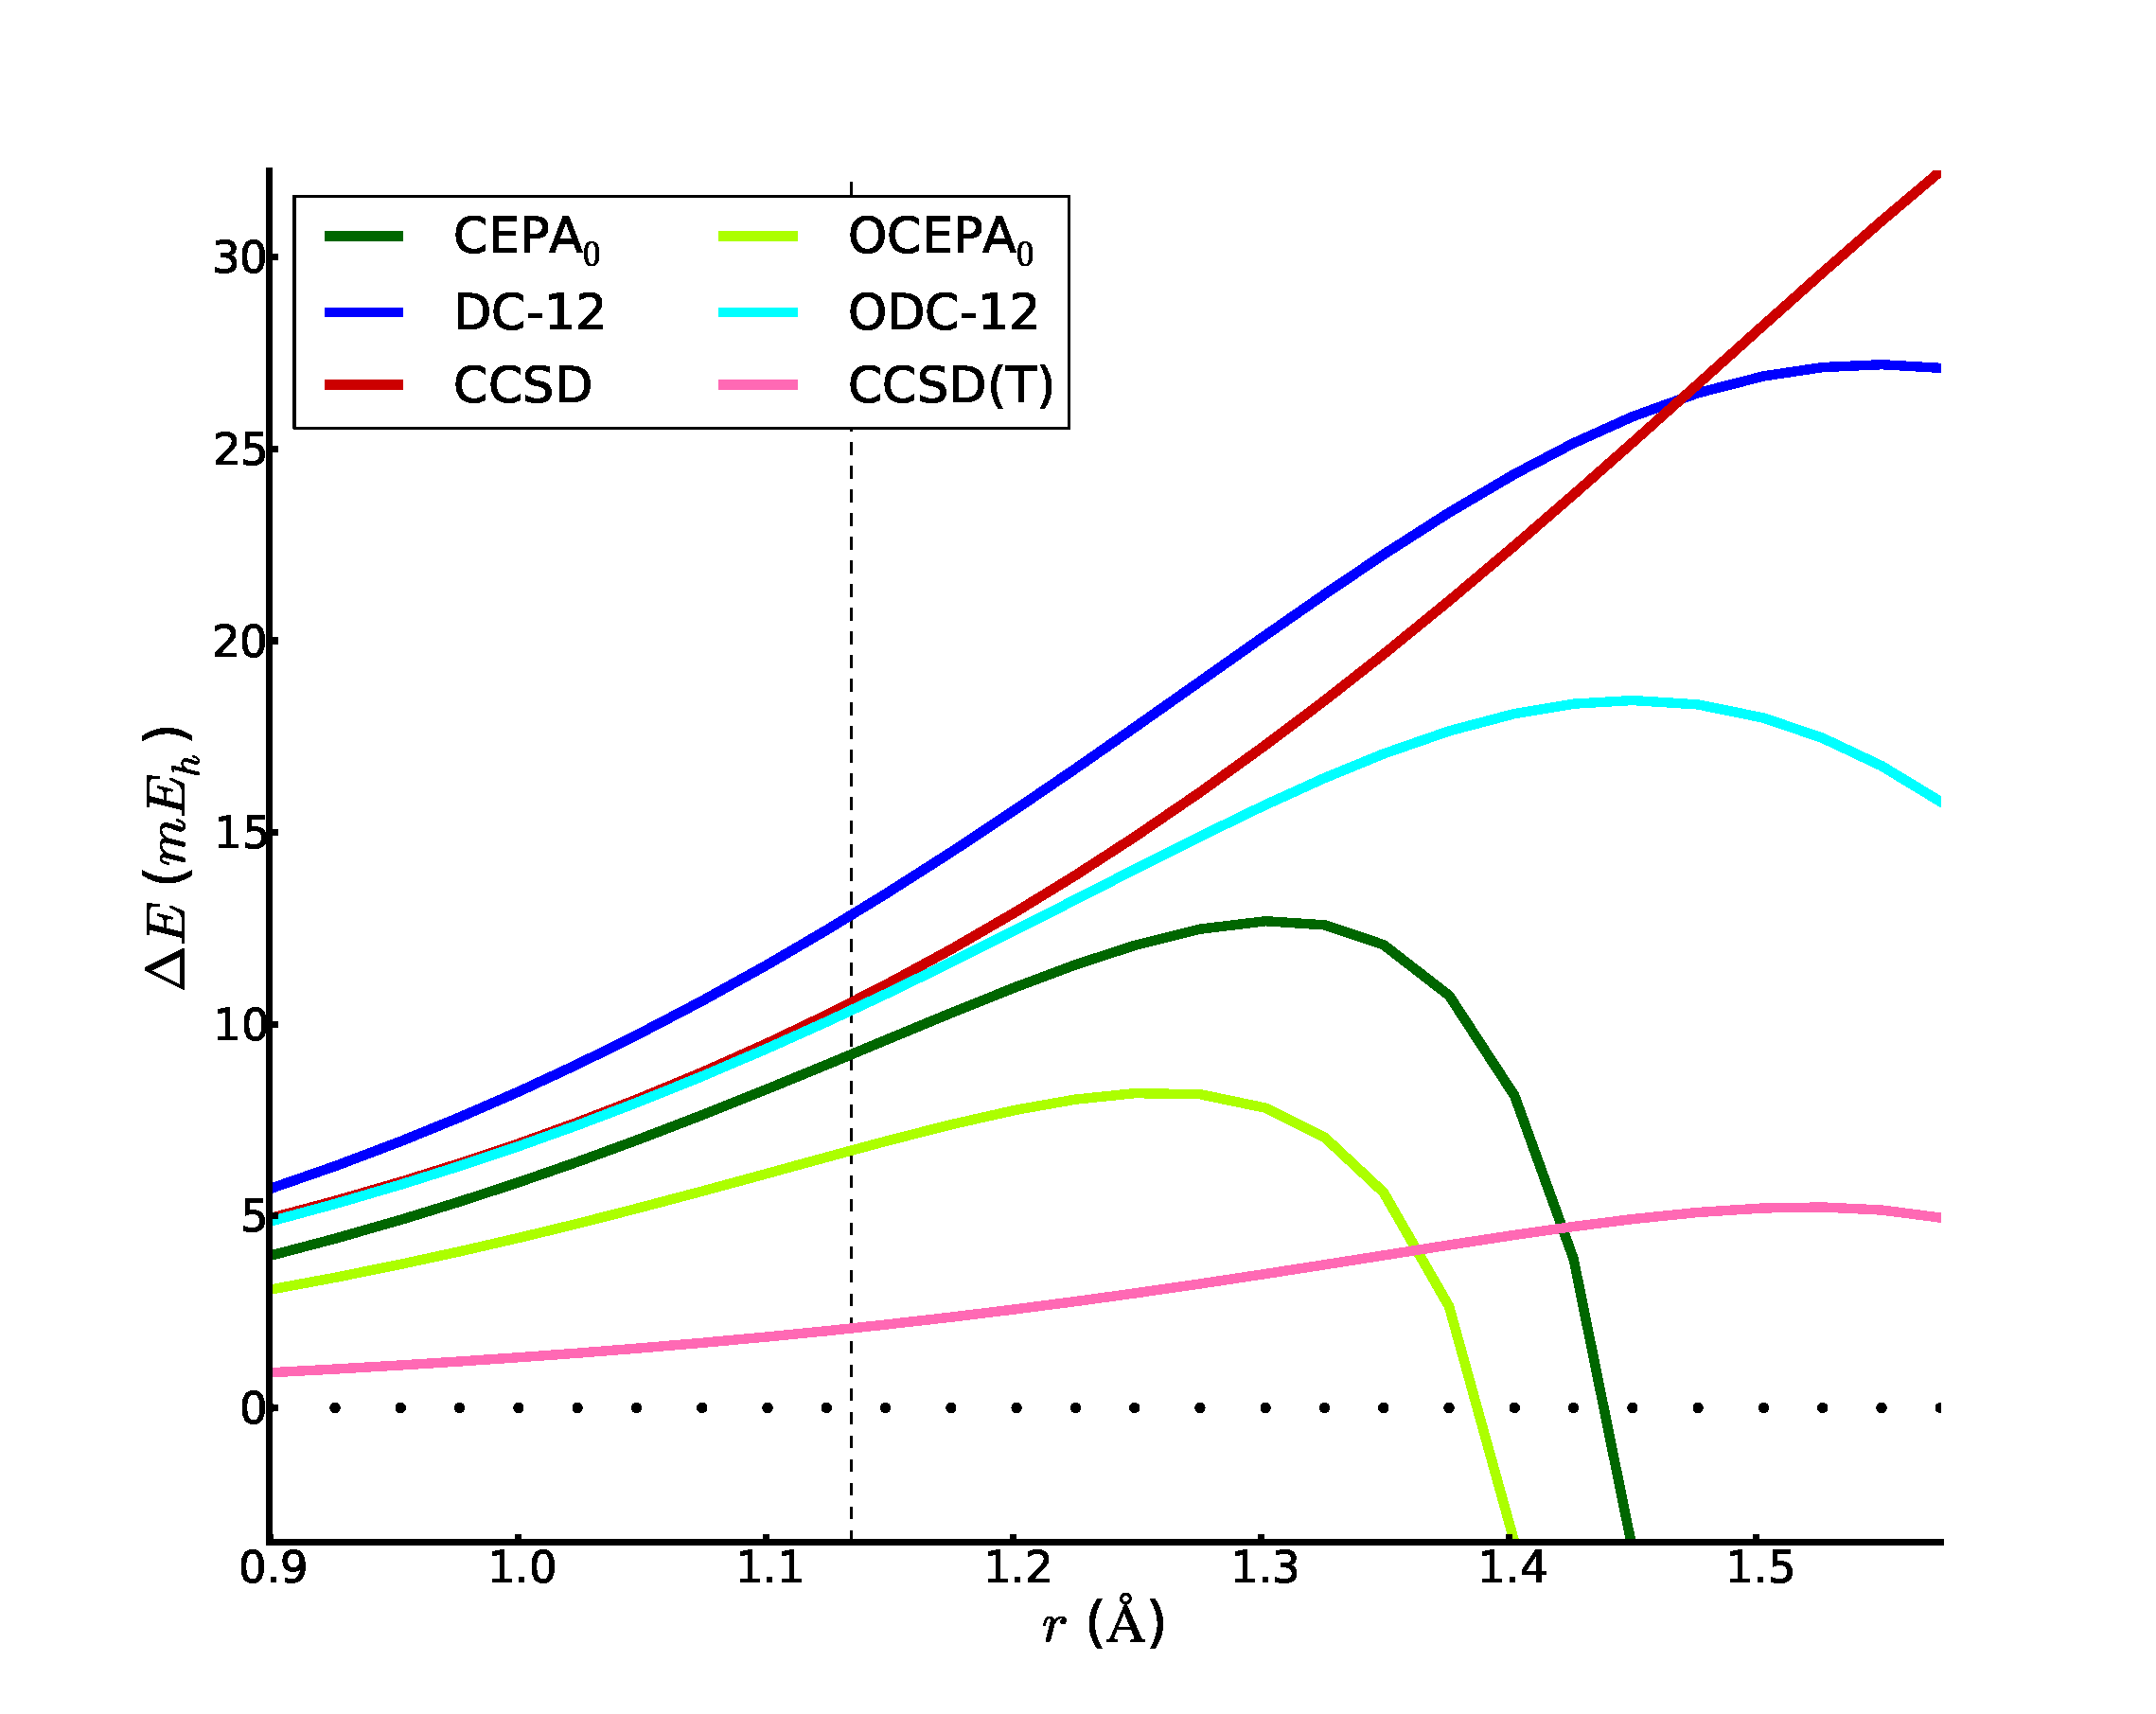
\includegraphics[width=0.8\textwidth]{figures/n2.pdf}
\end{figure}



\subsection{Covalent Bond Stretching in Diatomic Molecules}

Finally, we benchmark DCFT methods for covalent bond stretching.
Although accurate description of bond stretching demands the use of
multireference methods, our aim here is to explore the limits of DCFT away from
equilibrium.
For this purpose, we compute the energy as a function of bond distance for
diatomic molecules with single (HF and BH), double (BeO), and triple (\ce{N2})
bonds using the CEPA$_0$, OCEPA$_0$, DC-12, ODC-12, CCSD, and CCSD(T) methods.
We restrict ourselves to modest basis sets in order to use full CI (FCI) as a
reference, and plot the errors with respect to FCI ($\Delta E$) as a function of
internuclear distance for each molecule.
The relative performance of the methods is described below using non-parallelity
errors (NPE $=\Delta E_\mathrm{max}-\Delta E_\mathrm{min}$, \mhartree) computed
for specific bond distance ranges.


\paragraph{BH}

\Cref{bh-f} shows errors relative to FCI for the BH molecule.
DC-12 and CCSD increasingly overestimate the energy at larger internuclear
distances, whereas the CEPA$_0$ error curve is concave down.
Orbital optimization lowers the binding energy for OCEPA$_0$ even further
compared to CEPA$_0$, leading to large errors with respect to FCI for $r$(B--H)
> 1.5 \re, where \re is the FCI equilibrium bond distance (\re$=1.244$~\AA). At
1.87 \re, OCEPA$_0$ encounters convergence problems, which originate from
numerical instabilities due to the method's deficiencies in the description of
$N$-representability.
The ODC-12 method exhibits much more stable behavior with respect to bond
stretching in this case, fortuitously showing smaller errors and better
parallelity than CCSD(T).
For the range $[0.72\ \re, 2.47\ \re]$, the NPEs decrease in the order 
DC-12    (24~\mhartree) $>$
CEPA$_0$ (15) $>$
CCSD     (5) $>$
CCSD(T)  (3) $>$
ODC-12   (1).


\paragraph{HF}
Errors for HF bond stretching are plotted in \cref{hf-f}.
The $\Delta E$ values of CCSD and DC-12 increase as a function of $r$(H--F),
while CEPA$_0$ fortuitously maintains parallelity similar to CCSD(T) over the
range $[0.74\ \re, 1.94\ \re]$ ($\re = 0.929$~\AA).
OCEPA$_0$ increasingly overestimates the HF binding energy away from
equilibrium, failing to converge past 1.82 \re.
The ODC-12 method exhibits larger NPE than was observed for BH, and encounters
convergence problems past 1.94 \re.
CCSD(T) shows the best overall performance, with errors between 0 and
1~\mhartree.
In the range $[0.74\ \re, 1.94\ \re]$ the computed NPE values are:
DC-12    (15~\mhartree) $>$
CCSD     (7) $>$
ODC-12   (3) $>$
CEPA$_0$ (1) $\approx$
CCSD(T)  (1).
Recently, the orbital-optimized variants of CCSD(T) have been shown to yield
good performance for HF bond stretching.\cite{Bozkaya:2012p204114}

\paragraph{BeO}
The double bond of BeO presents a more challenging test for the single-reference
methods under consideration (\cref{beo-f}).
All methods but CCSD(T) show qualitatively similar error curves, with inflection
points near the FCI equilibrium ($\re=1.394$~\AA) and valleys/peaks around 0.6
\re/1.2 \re.
OCEPA$_0$ encounters convergence problems past 1.10 \re.
The ODC-12 method performs similarly to CCSD\@.
Overall, the NPEs for the range $[0.65\ \re, 1.10\ \re]$ decrease in the
following order:
DC-12    (29~\mhartree) $>$ 
CEPA$_0$ (24) $>$
ODC-12   (19) $>$
CCSD     (17) $>$
CCSD(T)  (3).

\paragraph{\ce{N2}}
\Cref{n2-f} depicts the errors relative to FCI for triple bond stretching in
\ce{N2}.
Here, OCEPA$_0$ fails to converge past 1.24 \re ($\re = 1.135$~\AA).
The ODC-12 method significantly overestimates the binding energy, possibly due
to the lack of three-body correlation effects, but shows much more stable
performance compared to methods other than CCSD(T).
NPEs in the range $[0.79\ \re, 1.39\ \re]$ decrease in the order:
CEPA$_0$ (802~\mhartree)\footnotemark $>$
\footnotetext{%
    CEPA$_0$ exhibits a vertical asymptote at 1.36 \re for N$_2$ stretching.
}
CCSD     (27) $>$
DC-12    (21) $>$
ODC-12   (14) $>$
CCSD(T)  (4).


\section{Conclusions}

We have presented the benchmark study of four density cumulant functional theory
(DCFT) methods (DC-06, DC-12, ODC-06, and ODC-12) developed recently in our
group.\cite{Simmonett:2010p174122,Sokolov:2012p054105,Sokolov:2013p024107,Sokolov:2013p204110}
Specifically we have compared the performance of DCFT to that of coupled
electron pair methods (CEPA$_0$ and OCEPA$_0$), as well as coupled-cluster
theory [CCSD and CCSD(T)] for predicting a variety of chemical properties
relevant to thermochemistry and kinetics, with a particular focus on open-shell,
electron-dense, and non-equilibrium systems.

Our results indicate that among the four DCFT methods, the best agreement with
available reference data is obtained for the ODC-12 method.
While all four DCFT formulations yield similar results for the description of
noncovalent interactions, DC-06, DC-12, and ODC-06 exhibit worse performance
than ODC-12 for thermodynamic and kinetic properties of reactions involving
open-shell molecules.
In particular, DC-06 and ODC-06 frequently encounter convergence problems that
originate from poor description of $N$-representability.
In comparing ODC-12 to other methods, several trends can be observed: 

(i) For all benchmark datasets, ODC-12 outperforms CCSD with errors smaller by
almost a factor of two, on average.
ODC-12 is also superior to CCSD for the description of single bond stretching in
BH and HF, although it does not converge for all bond distances.

(ii) The performance of ODC-12 and OCEPA$_0$ is comparable.
In particular, for hydrogen-transfer reaction barrier heights, the OCEPA$_0$
method yields smaller percent errors than ODC-12, whereas, for the radical
stabilization energies (RSE) and adiabatic ionization energies (AIE) in
electron-dense molecules, the ODC-12 method smaller standard deviations than
OCEPA$_0$.
For AIEs, ODC-12 gives smaller mean absolute deviations by almost a factor of
two.
ODC-12 also shows significantly smaller non-parallelity errors than OCEPA$_0$
for covalent bond stretching, and can be converged for a larger range of
distances for all diatomic molecules studied.

(iii) For the two most challenging datasets, RSE and AIE, the standard deviation
of ODC-12 and CCSD(T) are similar.
While CCSD(T) yields smaller mean absolute errors for the RSE database, the
ODC-12 method significantly outperforms CCSD(T) for the AIE test case.
However, for bond stretching ODC-12 is competitive with CCSD(T) only for the BH
dissociation and shows worse results for other molecules.

Overall, the data presented herein indicates that the ODC-12 method can be used
as an efficient $\mathcal{O}(n^6)$ alternative to CCSD, capable of predicting
thermodynamic and kinetic quantities that are competitive in accuracy with the
``gold-standard'' $\mathcal{O}(n^7)$ CCSD(T).
Although our current implementation of ODC-12 is far from optimal, the ODC-12
equations have reduced non-linearities compared to CCSD, which makes them more
amenable to parallel implementation.
The efficiency of ODC-12 can also greatly benefit from
spin-adaptation,\cite{Kutzelnigg:1999p2800,Kutzelnigg:2002p4787,Kutzelnigg:2010p433}
local
approximations,\cite{Werner:2003p8149,Taube:2005p837,Neese:2009p064103,Neese:2009p114108}
and density
fitting.\cite{Vahtras:1993p514,Hetzer:2000p9443,Schutz:2001p661,Werner:2003p8149}
Another important advantage of ODC-12 over CCSD is its stationarity, which makes
the computation of first-order properties and analytic gradients more efficient
and easily accessible.
In particular, ODC-12 has potential to be used for computing accurate response
properties which do not suffer from a lack of
gauge-invariance.\cite{Pedersen:1999p8318,Pedersen:2001p6983}
